 \documentclass[11pt,a4paper,twoside,pdf]{article}

% Paquetes (añade otros si los necesitas):
\usepackage{subcaption}
\usepackage[T1]{fontenc}
\usepackage[utf8]{inputenc}
\usepackage{csquotes}
\usepackage{mathabx}
\usepackage[pdftex,final]{graphicx}

% Style package
% Font Package (Palatino)
\usepackage{mathpazo}
% Packages for specific capabilities
\usepackage{rotating} % for text rotation in tables
\usepackage{multirow} % for multirow in tables
\usepackage{subfigure} % Place subfigures in figure environment
% Packages for specific symbols
\usepackage{amssymb}
\usepackage{amsmath}
\usepackage{amsfonts}
\usepackage{eurosym} % Euro symbol
\usepackage{bbding} % for \XSolidBrush
\usepackage{pifont} % for \ding{55} (a check mark)
 \usepackage{comment} 
\usepackage{stmaryrd}
\usepackage{latexsym}
\usepackage{soul}
\usepackage{array}
%\usepackage{marvosym}
\usepackage{epsfig}
\usepackage{graphics}
\usepackage{graphicx} 
\usepackage{amsfonts}
\usepackage{xspace}
\usepackage{float}  
\usepackage{multicol}
\usepackage{color}
\usepackage{booktabs}
\usepackage{xtab}
\usepackage[colorlinks=true,urlcolor=blue,linkcolor=blue,citecolor=blue]{hyperref}
\numberwithin{equation}{section}


\linespread{1.05}

% TFG en inglés:
%\usepackage[english]{babel} 
%\addto\captionsenglish{\renewcommand{\chaptername}{}}

% TFG en español:
\usepackage[spanish,es-nodecimaldot,es-tabla,es-lcroman,es-nosectiondot,
            es-noindentfirst]{babel}
\renewcommand\spanishchaptername{}

% Formato de la página:
\usepackage{fancyhdr}
\usepackage[top=2.88cm,bottom=2.97cm,left=2.95cm,right=2.95cm]{geometry}
\setlength{\parskip}{0.1cm}

% Pon aquí tus definiciones:

\newcommand{\dis}{\displaystyle}
%\sodef\an{}{.2em}{1em plus1em}{2em plus.1em minus.1em}

\begin{document}

% Portada %%%%%%%%%%%%%%%%%%%%%%%%%%%%%%%%%%%%%%%%%%%%%%%%%%%%%%%%%%%%%%%%%%%%%%

\pagestyle{empty}


\noindent
\begin{tabular}{r}

\includegraphics[width=8.8cm]{escudoUGRmonocromo.png} \\[-1.8ex]
\hspace{31mm}\vspace{-8mm}
\begin{tabular}{c}
\hline\\[-1ex]\hskip-2mm
{\bf Facultad de Ciencias}\hspace{18mm}
\end{tabular}
\end{tabular}

\large
\vspace{30mm}
\hspace{25mm}
\begin{tabular}{l}
GRADO EN F\'ISICA
\end{tabular}

\vspace{45mm}
\hspace{25mm}
\begin{tabular}{l}
TRABAJO FIN DE GRADO
\\[1.5ex]
\begin{tabular}{r} % o 'l', como prefieras
\hspace*{-4.3mm}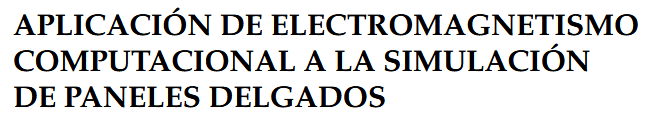
\includegraphics[width=12cm]{TFG/titulo.png} \\[-1.8ex]
\vspace{-8mm}
\end{tabular}
\end{tabular}
%
\vfill
\hspace{25mm}
\begin{tabular}{l}
Presentado por:
\\
{\bf D. Pablo Valdés Gámiz}
\\[3ex]
Curso Académico 2024/2025
\end{tabular}
%

\newpage
%

\begin{center}
{\bf Resumen}
\bigskip

\begin{minipage}{0.8\linewidth}
Este Trabajo de Fin de Grado presenta una implementación numérica del método discontinuo de Galerkin \cite{abstract1} para simular la propagación de ondas electromagnéticas en un entorno unidimensional. Tras una revisión crítica de distintos métodos numéricos—entre los que se encuentran diferencias finitas \cite{abstract2}, volúmenes finitos \cite{abstract3} y elementos finitos \cite{abstract4}—se justifica la elección del método \textit{DG-FEM} por su mejor adaptación a las necesidades de este proyecto. Se desarrollan las formulaciones débiles y fuertes de las ecuaciones de Maxwell adaptadas a este enfoque, incorporando materiales con permitividad y conductividad variables. El modelo se valida mediante el cálculo de los coeficientes de reflexión y transmisión de ondas al incidir sobre láminas delgadas, comparando los resultados obtenidos con simulaciones realizadas con la librería \textit{Scikit-rf} \cite{scikit}. Los resultados confirman la viabilidad del modelo y sientan las bases para futuras extensiones a sistemas multidimensionales.
\end{minipage}

\vfill

{\bf Abstract} 
\bigskip

\begin{minipage}{0.8\linewidth}
This Bachelor's Thesis presents a numerical implementation of the Discontinuous Galerkin method \cite{abstract1} to simulate the propagation of electromagnetic waves in a one-dimensional environment. Following a critical review of various numerical methods—including finite differences \cite{abstract2}, finite volumes \cite{abstract3}, and finite elements \cite{abstract4}—the choice of the \textit{DG-FEM} method is justified based on its better suitability for the project's requirements. Both the weak and strong formulations of Maxwell’s equations are developed within this framework, incorporating materials with variable permittivity and conductivity. The model is validated by computing the reflection and transmission coefficients of waves incident on thin layers, with results compared to simulations carried out using the \textit{Scikit-rf} library \cite{scikit}. The results confirm the model’s viability and lay the groundwork for future extensions to multidimensional systems.
\end{minipage}

\vfill

\end{center}
\newpage
% Indice %%%%%%%%%%%%%%%%%%%%%%%%%%%%%%%%%%%%%%%%%%%%%%%%%%%%%%%%%%%%%%%%%%%%%%%
%\newpage

\tableofcontents

% Texto %%%%%%%%%%%%%%%%%%%%%%%%%%%%%%%%%%%%%%%%%%%%%%%%%%%%%%%%%%%%%%%%%%%%%%%%
\newpage

\pagestyle{fancy}
\fancyhead[RO,LE]{\leftmark}
\fancyhead[LO,RE]{\thepage}
\fancyfoot{}

\section{Introducción}

La ciencia computacional se ha vuelto el medio principal para realizar avances científicos y la aplicación de diversos modelos matemáticos mediante simulaciones realizadas en ordenadores se ha vuelto indispensable para el análisis y predicción de fenómenos físicos \cite{computational}\cite{IEEComp}\cite{CompPhys}. Por otra parte, la manera en la que se define físicamente un fenómeno electromagnético es mediante las ecuaciones formuladas por James Clerk Maxwell en 1861 \cite{wikipedia}, las cuales describen y predicen cómo se comportan los campos eléctricos y magnéticos en el tiempo \cite{intromaxwell}. Al hablar de ecuaciones que evolucionan en el tiempo, la manera más natural de describir este comportamiento es mediante el uso de ecuaciones diferenciales, presentando las siguientes expresiones:

\begin{equation}
\left\{
\begin{aligned}
\vec{\nabla} \times \vec{E}\; &= -\frac{\partial \vec{B}}{\partial t} \\[10pt]
\vec{\nabla} \cdot \vec{E} \;\;&= \;\frac{\rho}{\varepsilon} \\[10pt]
\vec{\nabla} \times \vec{B}\; &= \;\mu \varepsilon \frac{\partial \vec{E}}{\partial t} + \mu \vec{J} \\[10pt]
\vec{\nabla} \cdot \vec{B}\;\; &= \;0
\end{aligned}
\right.
\label{eq:maxwell1}
\end{equation}
En estas expresiones $E$ se trata del campo eléctrico, $B$ del campo magnético y $J$ es la densidad de corriente eléctrica.
Este Trabajo de Fin de Grado (referido como \textit{TFG}, \textit{tesis} o \textit{proyecto} de aquí en adelante) está centrado en el estudio de un espacio unidimensional, así que será necesario escribir dichas ecuaciones para una dimensión (1D). Se escoge, por tanto, el siguiente conjunto de ecuaciones:
\begin{equation}
\left\{
\begin{aligned}
\frac{\partial E_y}{\partial x} &= -\frac{\partial B_z}{\partial t} \\[10pt]
\frac{\partial E_x}{\partial x} &= \frac{\rho}{\varepsilon} \\[10pt]
-\frac{\partial B_z}{\partial x} &= \mu \varepsilon \frac{\partial E_y}{\partial t} + \mu J_y \\[10pt]
\frac{\partial B_x}{\partial x} &= 0
\end{aligned}
\right.
\label{eq:Maxwell1D}
\end{equation}
Centrándose en estas ecuaciones, desde el ámbito de la física computacional, se pueden realizar simulaciones que sean capaces de reflejar situaciones reales mediante el uso de métodos numéricos. Estos métodos numéricos se encargan de representar ecuaciones diferenciales a través de aproximaciones, de manera que se obtengan soluciones que se acerquen lo máximo posible a las soluciones analíticas. Es necesaria la realización de aproximaciones a la hora de resolver las ecuaciones diferenciales debido al coste computacional que conllevaría resolverlas, si es que fuese siquiera posible \cite{numericos}. Así, se busca llegar a una solución aproximada, $\overline{u}_h(x,t)$ (escrita de aquí en adelante como $u_h$ por simplificar la notación), que tenga el menor error relativo posible con una teórica $u(x,t)$. 

Es muy usual que los métodos numéricos computacionales se basen en el uso de \textit{leyes de conservación} \cite{conservation}. Estas leyes se basan en principios físicos en los que se conservan distintas propiedades, como pueden ser el momento, la energía o la masa, y siguen la siguiente expresión: 

\begin{equation}
    \frac{\partial u(x,t)}{\partial t} + \nabla\cdot F(u)=S(u)
\end{equation}

En esta ecuación $u(x,t)$ es un vector de variables conservadas, $F(u)$ se trata de la matriz de vectores de flujo y $S(u)$ se corresponde a la función de residuos.

Una vez más, al simplificar los problemas a una dimensión, es necesario realizar la consecuente reducción de esta función a una dimensión (1D):

\begin{equation}
    \frac{\partial u(x,t)}{\partial t}+\frac{\partial f(u)}{\partial x}=g(x,t) \label{eqCL}
\end{equation}
Donde $f(u)$ es la función de flujo y $g(x,t)$ la de residuos.

Para un fenómeno electromagnético, por tanto, se pueden usar como leyes de conservación dos de las ecuaciones de Maxwell:
\begin{equation}
\left\{
\begin{aligned}
\frac{\partial E_y}{\partial x} &= -\frac{\partial B_z}{\partial t} \\[10pt]
-\frac{\partial B_z}{\partial x} &= \mu \varepsilon \frac{\partial E_y}{\partial t} + \mu J_y
\end{aligned}
\right.
\label{eq:maxwell}
\end{equation}

Una vez asentadas las bases sobre las que trabajan los distintos métodos numéricos, será necesario elegir con cuál trabajaremos. Observaremos cuatro posibles opciones: \textit{Método de diferencias finitas (FDM)}, \textit{Método del volumen finito (FVM)}, \textit{Método de los elementos finitos (FEM)} o \textit{Método Galerkin discontinuo de elementos finitos (DG-FEM)}. Tras haber escogido el que mejor se adapte a las necesidades del proyecto, solo será necesario implementarlo mediante código.
%\begin{figure}[h]
%\centering
%\includegraphics[width=8cm]{fig.png}				
%\caption{Si no es de elaboración propia, debe especificarse la fuente \cite{PYTHIA}. \label{figura1}}
%\end{figure}
%\noindent
\newpage
\section{Fundamento teórico}
En esta sección se tratará de exponer los puntos fuertes y las desventajas de cada uno de los métodos numéricos ya mencionados en la introducción.
\subsection{Método de diferencias finitas}
El método de las diferencias finitas \textit{(FDM)} es el más simple, ya que trata de aproximar la geometría del problema y representarla a través de un conjunto de puntos que se colocan como guía de lo que sería la forma física. Es necesario introducir aquí el concepto de \textit{malla} como una teselación del espacio de simulación en elementos, usualmente no superpuestos, que representan el espacio donde se representarán las soluciones computacionales del problema.

\begin{figure}[h]
\centering
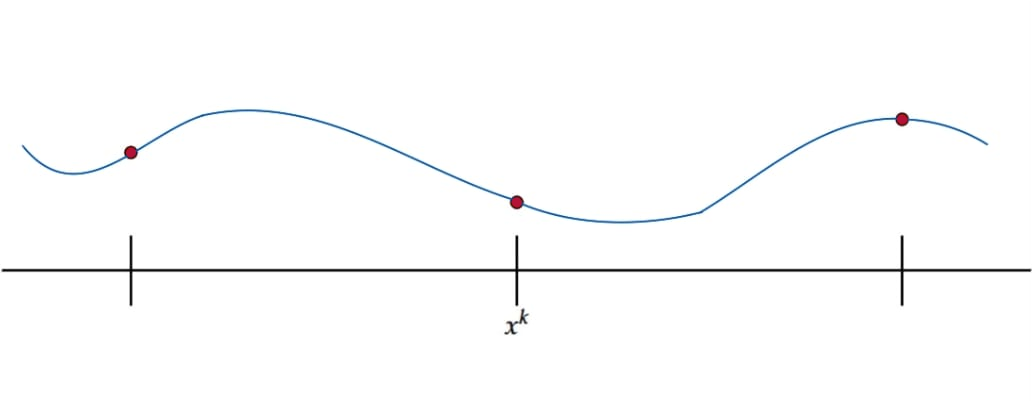
\includegraphics[width=10cm]{TFG/Fundamento/FDM.png}				
\caption{Representación gráfica del \textit{FDM} sobre una geometría cualquiera.}
\end{figure}
\noindent
Este planteamiento es simple de implementar si la geometría es sencilla, pero presenta como problema principal que, cuando se trata de geometrías que presentan discontinuidades, la forma en la que la malla que describe el problema se adapta a la geometría tiende a inducir errores elevados, ya que las soluciones aproximadas solo satisfacen las ecuaciones diferenciales de manera puntual.
\subsection{Método del volumen finito}
El funcionamiento de este método consiste en la división del dominio en celdas. Para cada una de estas celdas se establecerá la solución de la ecuación diferencial localmente como una "media". En otras palabras, se establece un valor medio aproximado de todos los puntos que pasan por esa celda, haciendo que, independientemente de cuál sea la forma real de la solución, su versión aproximada se verá representada como un valor constante, ver figura (\ref{FVM}). A esta solución también se la conoce como una solución de función interpoladora de orden cero. Adicionalmente, conviene mencionar el carácter local de la solución, lo cual crea un problema de doble evaluación en la frontera que requiere de la introducción de un `flujo' para definir la solución en fronteras entre elementos.


%\begin{figure}[H]
%\centering
%\includegraphics[width=10cm]{TFG/Fundamento/%FVM.png}				
%\caption{Representación gráfica del \textit{FVM} sobre una geometría cualquiera.} \label{FVM}
%\end{figure}

\noindent

A pesar de que este modelo es capaz de replicar geometrías complejas, la solución se ve limitada por el orden de la función interpoladora, que al ser de orden cero es constante. Este método es muy útil cuando las geometrías son sencillas debido a que es más fácil replicarlas dentro de las limitaciones del modelo, pero cuando estas geometrías se vuelven complejas, la limitación impuesta por la función interpoladora hace que se pierda resolución. En nuestro caso, buscamos un método que permita a la solución local adaptarse con mayor precisión que la que ofrece \textit{FVM}.

\begin{figure}[H]
\centering
\includegraphics[width=10cm]{TFG/Fundamento/FVM.png}				
\caption{Representación gráfica del \textit{FVM} sobre una geometría cualquiera.} \label{FVM}
\end{figure}
\subsection{Método de los elementos finitos}
La forma de operar bajo este método consiste en la división del cuerpo de la geometría en numerosos subdominios que tienen independencia entre sí. A estos subdominios son a los que se les llama \textit{elementos finitos}. Estos elementos finitos realizan una discretización del dominio original.  En cada elemento se identifican puntos clave llamados \textit{nodos}. Dos nodos se consideran adyacentes si pertenecen al mismo elemento. Además, los nodos situados en los bordes de un elemento pueden formar parte de varios elementos simultáneamente. 


\begin{figure}[h]
\centering
\includegraphics[width=10cm]{TFG/Fundamento/FEM2.png}				
\caption{Representación gráfica del \textit{FEM} sobre una geometría cualquiera.}
\end{figure}
\noindent
Este método, aunque útil bajo las circunstancias adecuadas, para el caso a estudiar en este proyecto tiene el gran problema de que su construcción es implícita en el tiempo. Que un método sea implícito en el tiempo quiere decir que el cálculo utilizado para hallar un valor futuro requiere utilizar ese mismo valor \cite{explicitorimplicit}:
\begin{equation}
    y_{n+1}=y_n+h\cdot f(t_{n+1},y_{n+1}) \notag
\end{equation}
Consecuentemente, para poder realizar ese cálculo se requiere resolver una ecuación adicional, a menudo no lineal, en cada paso, lo que, aunque aumenta enormemente el paso temporal que se puede utilizar, también incrementa el coste computacional del método.

Por otra parte, un método explícito permite calcular el valor de la función dependiente del tiempo a partir de valores ya conocidos en el paso temporal actual \cite{explicitorimplicit}:
\begin{equation}
    y_{n+1}=y_n+h\cdot f(t_{n+1},y_{n}) \notag
\end{equation}
Esto hace que cada paso se realice más rápidamente y de forma que el coste computacional sea menor. Es por esto que, teniendo en cuenta las necesidades de esta tesis, y que la estabilidad está garantizada para los problemas que se tratarán, se pretende utilizar un método explícito.


Se debe, por tanto, buscar realizar una modificación a este modelo que trate de salvaguardar su desventaja y que, además, intente adoptar las ventajas de los métodos anteriores.
\subsection{Método Galerkin discontinuo de elementos finitos}
Este método consistirá en subdividir el dominio con el que se pretende trabajar en una unión de elementos que no se superpongan:
\begin{equation}
   \Omega\cong\Omega_h=\bigcup_{k=1}^{K}D^k  \notag
\end{equation}
Donde $\Omega$ es el espacio físico, $\Omega_h$ es nuestra aproximación del espacio físico, pudiendo referirnos a él como espacio computacional, y $D^k$ son los elementos, no superpuestos, que unidos conforman el espacio computacional.

Esta subdivisión se realiza para que, al igual que en los métodos de elementos finitos y de volúmenes finitos, exista flexibilidad para representar geometrías de formas más complejas. 

Por otra parte, al contrario que durante el planteamiento del método de elementos finitos, para asegurar que la definición sea \textit{local} se duplica la cantidad de nodos existentes en las fronteras entre elementos, de modo que en cualquier frontera entre dos superficies cada frontera tenga su propio nodo, esto conlleva que, en términos de posiciones, $x_r^{k-1}=x_l^{k}$ y $x_r^{k}=x_l^{k+1}$.
\begin{figure}[h]
\centering
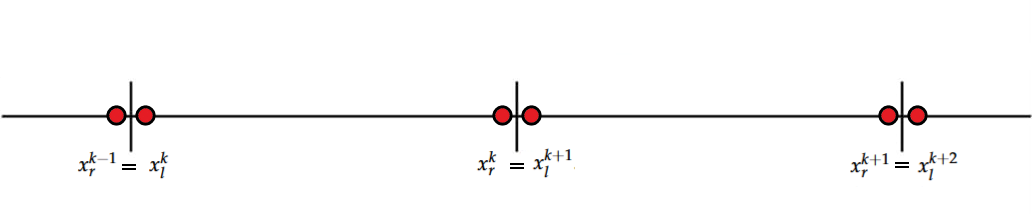
\includegraphics[width=14cm]{TFG/Fundamento/dgfem nodos.png}				
\caption{Representación gráfica del \textit{DG-FEM} sobre una geometría cualquiera.}
\end{figure}
\noindent

Siguiendo con las similitudes con el método de elementos finitos, se buscan realizar aproximaciones arbitrarias de alto orden. Para ello, se asume que en cada elemento la solución local aproximada sigue la expresión:

\begin{equation}
    u_h(x)=\sum^{N_p}_{n=1}b_n\psi_n(x)
\end{equation}
donde $\psi_n(x)$ introduce el uso de una función de base localmente definida y $N_p$ es el número de puntos interpolatorios o `grados de libertad', que en una dimensión se puede expresar como $N_p=p+1$, siendo $p$ el orden del polinomio.  En el caso más simple, y el usado para este desarrollo, se pueden tomar funciones de base lineales, como pueden ser los polinomios de Lagrange, $l(x)$, los cuales toman la siguiente forma:
\begin{equation}
    l_i^k(x)=\frac{x-x^{k+1-i}}{x^{k+i}-x^{k+1-i}} \notag
\end{equation}
 Sabiendo esto, se puede representar la función global usando aproximaciones locales polinómicas de alto orden, las cuales se expresan como:
\begin{equation}
    u(x,t)\cong u_h(x,t)=\bigoplus^K_{k=1}u^k_h(x,t)\notag
\end{equation}
donde
\begin{equation}
    u^k_h(x,t)=\sum^{N_p}_{i=1}u^k_h(x^k_i,t)l^k_i(x)\notag
\end{equation}
En la cual $l^k_i(x)$ se trata de la \textit{función de aproximación} o \textit{trial}.

Una vez se ha llegado hasta aquí, se busca encontrar una aproximación $u_h$ a la solución $u$ de la ley de conservación general escalar expuesta previamente en (\ref{eqCL}). Con este objetivo, se forma el residuo local de los elementos k=1,...,K:
\begin{equation}
    x\in D^k: \mathcal{R}_h^k(x,t)=\frac{\partial u^k_h(x,t)}{\partial t} + \frac{\partial f^k_h(u)}{\partial x} - g^k_h(x,t) \label{residuo}
\end{equation}
De aquí en adelante se omitirán las dependencias con respecto a las distintas variables de $l_j^k$, $\mathcal{R}_h^k$, $u^k_h$, $f^k_h$ y $g^k_h$ por simplicidad a la hora de realizar desarrollos.

Este residuo debe ser ortogonal a todas las funciones de base, anulándose localmente de la siguiente manera:
\begin{equation}
    \int_{D^k} \mathcal{R}_h^k\;l_j^kdx=0, \;\;\;\;\; j=1,...,N_p \;\;\;\;\;\; k=1,...K \label{residuo2}
\end{equation}
En esta expresión, a $l_j^k$ se la denomina \textit{función de prueba} o \textit{test}. En el método de Galerkin, una función \textit{test} es una función que se utiliza para proyectar o filtrar la ecuación diferencial que se está resolviendo. En lugar de exigir que la ecuación se cumpla punto por punto (\textit{forma fuerte}), se exige que se cumpla en promedio contra una serie de funciones \textit{test}.

Formalmente, una función \textit{test} es un elemento del espacio de funciones contra el cual se proyecta el residuo de la ecuación para obtener una \textit{formulación débil}.

Esta es una de las bases de un esquema \textit{DG-FEM} nodal. Sin embargo, aparecen dos problemas. El primero es que los elementos están desconectados porque la formulación \textit{DG} no impone continuidad entre ellos, haciendo que los residuos solo puedan estar definidos de forma local. Mientras que el segundo es que, como las fronteras entre elementos están compartidas por dos elementos, se necesita imponer una condición que asegure la unicidad de la función.

Para solucionar el primer problema que se presenta se trata de conectar elementos mediante el teorema de Gauss:
\begin{equation}
    \int_{D^k} \mathcal{R}_h^k\;l_j^kdx=\int_{D^k}\left[\frac{\partial u^k_h}{\partial t}l_j^k + \frac{\partial f^k_h}{\partial x}l_j^k - g^k_hl_j^k\right]dx=-\oint_{\partial D^k}\hat{n}\cdot f_h^kl_j^kdx \notag
\end{equation}
Esta última integral de frontera en 1D toma el siguiente resultado:
\begin{equation}
  \oint_{\partial D^k}\hat{n}\cdot f_h^kl_j^kdx=\left[f_h^kl_j^k\right]^{x_l^k}_{x_r^k}=f_h^k(x_r^k)\delta_{N_{p} j}- f_h^k (x_l^k) \delta_{1j} \notag 
\end{equation}


Habiendo llegado hasta aquí, falta solucionar el problema de la unicidad de la solución. Para solucionarlo, es suficiente introducir un flujo numérico, $f^*$, como el único valor a usar en la frontera y siendo obtenido mediante la combinación de información de ambos elementos. Para realizar esto, existen dos formulaciones, la construcción débil:
\begin{equation}
\int_{D^k} \frac{\partial u_h^k}{\partial t} l_j^k - f_h^k \frac{dl_j^k}{dx} - g^k_h l_j^k \, dx = - \left[ f^* l_j^k \right]_{x^k}^{x^{k+1}} ,  \label{weak}
\end{equation}
y la construcción fuerte aplicando de nuevo el teorema de Gauss:
\begin{equation}
\int_{D^k} \mathcal{R}_h\;l_j^k\;dx=\left[(f_h^k-f^*)l_j^k\right]^{x^{k+1}}_{x^{k}}.     \label{strong}
\end{equation}
De esta manera, mediante la introducción de un flujo numérico, quedaría solucionado el problema de la conexión de elementos, haciéndose más claro al observar que tanto el elemento \(D^k\) como el elemento $D^{k+1}$ dependen de la evaluación del flujo en el punto $x^{k+1}$, compartido entre los dos elementos.

Es importante destacar, por tanto, que la elección del flujo numérico es una parte fundamental y central a la hora de aplicar el método y será donde se puedan aplicar los conocimientos de la dinámica de cada problema. Más adelante se discutirá cómo se ha designado dicho flujo para los casos a tratar en esta tesis.

Partiendo de esto, se puede generar un sistema lineal local mediante la introducción de la matriz de masa ($\mathcal{M}$) y la de rigidez ($\mathcal{S}$), las cuales tienen la siguiente forma:
\begin{equation}
    \mathcal{M}^k_{ij}=\int_{D^k} l_i^k\;l_j^k\;dx, \;\;\;\; \mathcal{S}^k_{ij}=\int_{D^k}l_i^k\frac{dl_j^k}{dx}dx \notag
\end{equation}
Cabe destacar que la matriz de masa se trata, por tanto, de la integral de la función \textit{trial} ($l_i^k$) por la función \textit{test} ($l_j^k$), mientras que la de rigidez se trata de la integral del producto de la función \textit{trial} por la derivada espacial de la función \textit{test}. Es importante explicar que las funciones de base de forma habitual no tendrían por qué ser siempre las mismas entre \textit{trial} y \textit{test}, el que lo sean es una implicación del método de Galerkin utilizado.

Quedando la forma débil:
\begin{equation}
    \frac{du_h^k}{dt}=-\left( \mathcal{M}^k \right)^{-1}\left[l^k_j\;f^*\right]^{x_r^k}_{x_l^k}+\left( \mathcal{M}^k \right)^{-1}\left(\mathcal{S}^k\right)^Tf_h^k+g_h^k \label{weaktime} 
\end{equation}
y la forma fuerte:
\begin{equation}
\begin{split}
\frac{du_h^k}{dt} = \left( \mathcal{M}^k \right)^{-1}\left[(f^k_h-f^*)\;l^k_j\right]^{x_r^k}_{x_l^k} 
  +\left( \mathcal{M}^k \right)^{-1} \left(\mathcal{S}^k\right) f_h^k + g_h^k \label{strongtime}
\end{split}
\end{equation}
Estas dos ecuaciones son resolubles mediante métodos numéricos de ecuaciones diferenciales ordinarias. 

Así que, finalmente, hemos logrado construir un método que, aunque similar a los métodos de elementos  (\textit{FEM}) y de volumen finito (\textit{FVM}), supera las limitaciones que traen consigo dichos métodos. Como se estableció durante la introducción de \textit{FEM}, para el estudio a realizar se necesita que la construcción no sea implícita, objetivo que se ha logrado al introducir la matriz de masa de forma local en vez de global, imponiendo un esquema semidiscreto que es explícito. No solo se soluciona el problema inherente al \textit{FEM}, sino que se soluciona la limitación del \textit{FVM} pudiendo lograr precisión a altos órdenes a través del establecimiento de una base de elementos locales. Estas ventajas se consiguen a su vez sin perder la flexibilidad que otorga la elección de flujo también presente en \textit{FEM}.
\newpage
\section{Metodología}
\subsection{Desarrollo de las ecuaciones de Maxwell}
%Desarrollo de las dobles integrales y como se introduce J en todo esto
Una vez escogido el método a seguir, es decir, \textit{DG-FEM}, se debe tratar de adaptar a las necesidades de este \textit{TFG}. Al estar esta tesis enfocada al estudio de ondas electromagnéticas, es evidente que el foco recaerá sobre las ecuaciones de Maxwell tal y como se explica en la introducción. Sin embargo, se deben tratar de expresar dichas ecuaciones de manera que sean congruentes con la forma requerida por discontinuo Galerkin. A lo largo de este apartado se tratará de transformar las ecuaciones (\ref{eq:maxwell}) para que tengan la forma requerida. Para simplificar el proceso se trabajará bajo un sistema donde, inicialmente, $J$ sea nula y, además, al trabajar en una dimensión (1D), $E_y$ se expresará simplemente como $E$ y $B_z$ como $B$, de forma que el punto de partida es el siguiente:
\begin{equation}
\frac{\partial E}{\partial x} +\frac{\partial B}{\partial t}=\mu\frac{\partial H}{\partial t}+\frac{\partial E}{\partial x}=0 \label{eq31}
\end{equation}
\begin{equation}
\frac{\partial B}{\partial x} + \mu \varepsilon \frac{\partial E}{\partial t}=0\Rightarrow\varepsilon \frac{\partial E}{\partial t}+\frac{\partial H}{\partial x} =0  \label{eq32}
\end{equation}
Al haber expresado así las ecuaciones, es apreciable que tienen la misma forma que el residuo presente en (\ref{residuo}), así que se puede partir del siguiente paso planteado durante el fundamento teórico, es decir, desarrollar la integral (\ref{residuo2}). En el caso presente se tienen dos ecuaciones a las que realizarles el desarrollo; en primer lugar se realizará para (\ref{eq31}), es decir, se obtendrá la derivada temporal de $H$, y posteriormente se realizará para (\ref{eq32}), es decir, se obtendrá la derivada temporal de $E$.
\subsubsection{Ecuación diferencial temporal de \textit{H}}
Para comenzar con el desarrollo, con fin de obtener la derivada temporal de H, se introduce, tal y como se ha explicado, la expresión (\ref{eq31}) como residuo en la ecuación (\ref{residuo2}), resultando en:
\begin{equation}
    \int^{x^k_r}_{x^k_l}\left(\mu\frac{\partial H}{\partial t}+\frac{\partial E}{\partial x}\right)l_j^k(x)\;dx=0 \notag
\end{equation}
Sobre esta ecuación se integra por partes:
\begin{align}
    \int^{x^k_r}_{x^k_l}\mu\frac{\partial H}{\partial t}l_j^k\;dx 
    + \int^{x^k_r}_{x^k_l}\frac{\partial E}{\partial x} l_j^k\;dx 
    = \int^{x^k_r}_{x^k_l}\mu\frac{\partial H}{\partial t}l_j^k\;dx \notag
    \; + \left[E\;l_j^k\right]^{x^k_r}_{x^k_l}
    - \int^{x^k_r}_{x^k_l}E\frac{dl_j^k}{dx}\;dx = 0 \notag
\end{align}
\begin{equation}
        \text{Con}
\left\{
\begin{aligned}
u &= l_j^k \;\;\;\;\;\;\; du=\frac{dl_j^k}{dx} \\
dv &= \frac{\partial E}{\partial x}\;\;\;\;\;\;\; v=\int\frac{\partial E}{\partial x}\;dx=E
\end{aligned}
\right. \notag
\end{equation}
Esta relación se puede expresar por tanto de la siguiente forma:
\begin{equation}
\int^{x^k_r}_{x^k_l}\left(\mu\frac{\partial H}{\partial t}l_j^k\;-E\frac{dl_j^k}{dx}\;\right)dx=-\left[E\;l_j^k\right]^{x^k_r}_{x^k_l}
    \notag
\end{equation}
Aquí es posible reescribir la parte de la derecha de la integral como una integral de superficie, obteniendo así
\begin{equation}
 \int^{x^k_r}_{x^k_l}\left(\mu\frac{\partial H}{\partial t}l_j^k\;-E\frac{dl_j^k}{dx}\right)dx=-\oint^{x^k_r}_{x^k_l}\hat{n}\cdot E\;l_j^k\;dx
    \notag   
\end{equation}
donde $\hat{n}$ representa la normal local que apunta hacia fuera. El uso de una integral de superficie puede no parecer un paso intuitivo que dar; sin embargo, hace que las generalizaciones sean muy naturales. Además, al estar tratando de una única dimensión, y como hemos definido que la normal del elemento apunta hacia el exterior, en la frontera derecha $\hat{n}$ tomará el valor unidad positivo, mientras que en la frontera izquierda tomará el valor unidad negativo.

Para completar el esquema, se debe recordar que dos elementos vecinos contarán, cada uno, con un grado de libertad definido sobre la misma frontera, es decir, $x^k_r=x^{k+1}_l$. Así que, llegados a este punto, se tendrán dos soluciones, lo cual introduce un problema de doble evaluación que necesitamos resolver. Es por esto que se introduce el \textit{flujo numérico}, $E^*$. La elección del flujo es de suma importancia y la discusión de la misma se hará tras haber finalizado con el desarrollo de las ecuaciones de Maxwell. En este caso, se introducirá el flujo en la parte derecha de la ecuación, con el fin de conectar los elementos. De esta forma, se habrá llegado a la construcción débil dada en (\ref{weak}) pero para la ecuación de Maxwell a utilizar:
\begin{equation}
    \int^{x^k_r}_{x^k_l}\left(\mu\frac{\partial H}{\partial t}l_j^k\;-E\frac{dl_j^k}{dx}\right)dx=-\left[E^*\;l_j^k\right]^{x^k_r}_{x^k_l}=-\oint^{x^k_r}_{x^k_l}\hat{n}\cdot E^*\;l_j^k\;dx
    \notag    
\end{equation}

A continuación, el desarrollo se centra en la parte de la izquierda del igual, volviendo a integrar por partes dicha expresión:
\begin{equation}
\int^{x^k_r}_{x^k_l}\mu\frac{\partial H}{\partial t}l_j^k\;dx-\int^{x^k_r}_{x^k_l}E\frac{dl_j^k}{dx}\;dx=\int^{x^k_r}_{x^k_l}\mu\frac{\partial H}{\partial t}l_j^k\;dx \;-\left[E\;l_j^k\right]^{x^k_r}_{x^k_l}\; + \int^{x^k_r}_{x^k_l}\frac{\partial E}{\partial x}l_j^kdx
    \notag    
\end{equation}
\begin{equation}
        \text{Con}
\left\{
\begin{aligned}
u &= E \;\;\;\;\;\;\; du=\frac{\partial E}{\partial x}dx \\
dv &= \frac{d l_j^k}{dx}\;\;\;\;\;\;\; v=\int\frac{dl_j^k}{d x}\;dx=l_j^k
\end{aligned}
\right. \notag
\end{equation}
Reagrupando términos y juntando esta expresión con la del lado derecho, se llega a:
\begin{equation}
    \int_{x^k_l}^{x^k_r}\left(\mu\frac{\partial H}{\partial t}l_j^k + \frac{\partial E}{\partial x}l_j^k\right)dx 
= \left[(E - E^*)\, l_j^k\right]_{x^k_l}^{x^k_r} \
= \displaystyle \oint_{x^k_l}^{x^k_r} \hat{n} \cdot (E - E^*)\, l_j^k\, dx
\end{equation}
siendo esta la forma fuerte a la que se llegó en (\ref{strong}) para la ecuación de Maxwell que se está tratando.

Una vez llegados a este punto se pueden sustituir los campos eléctricos y magnéticos en (\ref{weaktime}) y (\ref{strongtime}) para obtener la expresión de las ecuaciones diferenciales temporales para la forma fuerte y débil en función de la matriz de masa y la matriz de rigidez. 

La ecuación diferencial temporal de la \textit{forma débil} es:
\begin{equation}
    \frac{dH_h^k}{dt}=\frac{1}{\mu^k}\left(-\left( \mathcal{M}^k \right)^{-1}\left[(E^*)\;l_j^k\right]^{x^k_r}_{x^k_l}+\left( \mathcal{M}^k \right)^{-1}\left(\mathcal{S}^k\right)^TE_h^k\right)\notag
\end{equation}
Y para la \textit{forma fuerte}:
\begin{equation}
\begin{split}
\frac{dH_h^k}{dt} = \frac{1}{\mu^k}\left(\left( \mathcal{M}^k \right)^{-1}  \left[(E^k_h-E^*)\;l_j^k\right]^{x^k_r}_{x^k_l} 
  +\left( \mathcal{M}^k \right)^{-1} \left(\mathcal{S}^k\right) E_h^k\right)
\end{split}\notag
\end{equation}
Parecería que el desarrollo ya está completo dado que se ha llegado a las ecuaciones temporales que se tenían como referencia en el fundamento teórico; sin embargo, estas no serán las ecuaciones exactas que se harán evolucionar en el código. Estas expresiones se pueden hacer más flexibles añadiendo una nueva matriz a la que se llamará \textit{matriz de derivadas} y se representará como $\mathcal{D}_r$.

Esta matriz de derivación se define como:
\begin{equation}
    \mathcal{D}_{r,(ij)}=\left.\frac{dl_j}{dr}\right|_{r_i}
\end{equation}
El producto de esta nueva matriz con la matriz de masas es lo que centra el foco sobre la matriz de diferenciación:
\begin{equation}
    \left(\mathcal{MD}_r\right)_{ij}=\sum^{N_p}_{n=1}\mathcal{M}_{in}\mathcal{D}_{r,(nj)}=\sum^{N_p}_{n=1}\int^1_{-1}l_i(r)l_n(r)\left.\frac{dl_j}{dr}\right|_{r_n}\;dr= \notag
\end{equation}
\begin{equation}
    =\int^1_{-1}l_i(r)\sum^{N_p}_{n=1}\left.\frac{dl_j}{dr}\right|_{r_n}l_n(r)\;dr=\int_{-1}^1l_i^k(x)\frac{dl_j^k(x)}{dx}dx=\int_{x^k_l}^{x^k_r}l_i(x)\frac{dl_j(x)}{dx}dx  =\mathcal{S}_{ij}
    \notag
\end{equation}
En otras palabras, se tiene la identidad:
\begin{equation}
    \mathcal{MD}_r=S\notag
\end{equation}
Con esta información, se puede expresar la derivada temporal de $H$ en su \textit{forma fuerte}, que es la que se utilizará en el código, como:
\begin{comment}

\begin{equation}
       \frac{dH_h^k}{dt}=\frac{1}{J^k\mu^k}\left(-\mathcal{M}^{-1}\left[l^k(x)E^*\right]^{x_r^k}_{x_l^k}\;-\mathcal{D}_rE^k_h\right)\notag \notag
\end{equation}

Y siguiendo con la \textit{forma fuerte}:
    
\end{comment}
\begin{equation}
    \frac{dH_h^k}{dt}=\frac{1}{\mathcal{J}^k\mu^k}\left(\mathcal{M}^{-1}\left[(E^k_h-E^*)\;l_j^k\right]^{x_r^k}_{x_l^k}\;-\mathcal{D}_rE^k_h\right)
    \label{eqdH}
\end{equation}
En esta ecuación $\mathcal{J}^k$ se trata simplemente del Jacobiano del elemento \textit{k-ésimo}, utilizado para llevar el dominio físico al de referencia. 
\newpage
\subsubsection{Ecuación diferencial temporal de \textit{E}}
El proceso para la derivada temporal de E es completamente análogo al de H. Se introduce, por tanto, la ecuación (\ref{eq32}) en la fórmula del residuo tal y como se hizo previamente:
\begin{equation}
    \int^{x^k_r}_{x^k_l}\left(\varepsilon\frac{\partial E}{\partial t}+\frac{\partial H}{\partial x}\right)l_j^k\;dx=0 \notag
\end{equation}
Sobre esta ecuación se integra por partes:
\begin{align}
    \int^{x^k_r}_{x^k_l}\varepsilon\frac{\partial E}{\partial t}l_j^k\;dx 
    + \int^{x^k_r}_{x^k_l}\frac{\partial H}{\partial x} l_j^k\;dx = \int^{x^k_r}_{x^k_l}\varepsilon\frac{\partial E}{\partial t}l_j^k\;dx \notag  + \left[H\;l_j^k\right]^{x^k_r}_{x^k_l}
    - \int^{x^k_r}_{x^k_l}H\frac{dl_j^k}{dx}\;dx = 0 \notag
\end{align}
\begin{equation}
        \text{Con}
\left\{
\begin{aligned}
u &= l_j^k \;\;\;\;\;\;\; du=\frac{dl_j^k}{dx} \\
dv &= \frac{\partial H}{\partial x}\;\;\;\;\;\;\; v=\int\frac{\partial H}{\partial x}\;dx=H
\end{aligned}
\right. \notag
\end{equation}
Esta relación se puede expresar, por tanto, de la siguiente forma:
\begin{equation}
\int^{x^k_r}_{x^k_l}\left(\varepsilon\frac{\partial E}{\partial t}l_j^k\;-H\frac{dl_j^k}{dx}\;\right)dx=-\left[H\;l_j^k\right]^{x^k_r}_{x^k_l}
    \notag
\end{equation}
En función de la integral de superficie queda como:
\begin{equation}
 \int^{x^k_r}_{x^k_l}\left(\varepsilon\frac{\partial E}{\partial t}l_j^k\;-H\frac{dl_j^k}{dx}\right)dx=-\oint^{x^k_r}_{x^k_l}\hat{n}\cdot H\;l_j^k\;dx
    \notag   
\end{equation}

De nuevo, se introduce el flujo en el elemento de la parte derecha, con el fin de conectar los elementos. De esta forma se habrá llegado a la construcción débil dada en (\ref{weak}) pero para la ecuación de Maxwell correspondiente:
\begin{equation}
    \int^{x^k_r}_{x^k_l}\left(\varepsilon\frac{\partial E}{\partial t}l_j^k\;-H\frac{dl_j^k}{dx}\right)dx=-\left[H^*\;l_j^k\right]^{x^k_r}_{x^k_l}=-\oint^{x^k_r}_{x^k_l}\hat{n}\cdot H^*\;l_j^k\;dx
    \notag    
\end{equation}

Se vuelve a integrar por partes la parte izquierda del igual:
\begin{equation}
\int^{x^k_r}_{x^k_l}\varepsilon\frac{\partial E}{\partial t}l_j^k\;dx-\int^{x^k_r}_{x^k_l}H\frac{dl_j^k}{dx}\;dx=\int^{x^k_r}_{x^k_l}\varepsilon\frac{\partial E}{\partial t}l_j^k\;dx \;-\left[H\;l_j^k\right]^{x^k_r}_{x^k_l}\; + \int^{x^k_r}_{x^k_l}\frac{\partial H}{\partial x}l_j^kdx
    \notag    
\end{equation}
\begin{equation}
        \text{Con}
\left\{
\begin{aligned}
u &= H \;\;\;\;\;\;\; du=\frac{\partial H}{\partial x}dx \\
dv &= \frac{d l_j^k}{dx}\;\;\;\;\;\;\; v=\int\frac{dl_j^k}{d x}\;dx=l_j^k
\end{aligned}
\right. \notag
\end{equation}
Reagrupando términos y juntando esta expresión con la del lado derecho se llega a la \textit{forma fuerte}:
\begin{equation}
    \int_{x^k_l}^{x^k_r}\left(\varepsilon\frac{\partial E}{\partial t}l_j^k + \frac{\partial H}{\partial x}l_j^k\right)dx 
= \left[(H - H^*)\, l_j^k\right]_{x^k_l}^{x^k_r} = \displaystyle \oint_{x^k_l}^{x^k_r} \hat{n} \cdot (H - H^*)\, l_j^k\, dx
\end{equation}

Finalmente, la ecuación diferencial temporal de la \textit{forma débil} es:
\begin{equation}
    \frac{dE_h^k}{dt}=\frac{1}{\varepsilon^k}\left(-\left( \mathcal{M}^k \right)^{-1}\left[H^*\;l_j^k\right]^{x^k_r}_{x^k_l}+\left( \mathcal{M}^k \right)^{-1}\left(\mathcal{S}^k\right)^TH_h^k\right)\notag
\end{equation}
Y la de la \textit{forma fuerte}:
\begin{equation}
\begin{split}
\frac{dE_h^k}{dt} = \frac{1}{\varepsilon^k}\left(\left( \mathcal{M}^k \right)^{-1}  \left[(H^k_h-H^*)\;l_j^k\right]^{x^k_r}_{x^k_l} 
  +\left( \mathcal{M}^k \right)^{-1} \left(\mathcal{S}^k\right) H_h^k\right)
\end{split}\notag
\end{equation}
Como en el apartado anterior, la ecuación diferencial de \textit{forma fuerte}, que es la que se usa principalmente, se adapta para que incluya a la matriz de diferenciación, $\mathcal{D}_r$:
\begin{comment}

\begin{equation}
       \frac{dH_h^k}{dt}=\frac{1}{J^k\mu^k}\left(-\mathcal{M}^{-1}\left[l^k(x)E^*\right]^{x_r^k}_{x_l^k}\;-\mathcal{D}_rE^k_h\right)\notag \notag
\end{equation}

Y siguiendo con la \textit{forma fuerte}:
    
\end{comment}
\begin{equation}
    \frac{dE_h^k}{dt}=\frac{1}{\mathcal{J}^k\varepsilon^k}\left(\mathcal{M}^{-1}\left[(H^k_h-H^*)\;l_j^k\right]^{x_r^k}_{x_l^k}\;-\mathcal{D}_rH^k_h\right)
    \label{eqdE}
\end{equation}
Una vez se ha completado el desarrollo necesario para las ecuaciones de Maxwell para llegar a las funciones que se utilizan computacionalmente, se busca elegir y justificar el \textit{flujo numérico} a usar.
\subsection{Elección del flujo numérico}
Como se ha mencionado previamente, la elección del flujo es muy importante ya que este es responsable de la combinación de las soluciones locales en una global. A la hora de elegir el flujo, una condición natural que se debe cumplir es que el modelo resultante debe ser consistente. Esto quiere decir que la solución exacta debe satisfacer la construcción realizada al definir el espacio de elementos.

Una solución que asegura estas condiciones se trataría de un \textit{flujo central simple}:
\begin{equation}
    \hat{n}\cdot F^*(q^-,q^+)=\frac{1}{2}\left[F(q^-)+F(q^+)\right]
\end{equation}
Donde $F^*$ refiere al flujo, ya sea $E^*$ o $H^*$, mientras que $q^-$ refiere a la solución local y $q^+$ a la del elemento vecino. La variable $q$ puede hacer referencia al campo $H$ o $E$ dependiendo del flujo $E^*$ o $H^*$ respectivamente.

La ventaja principal de elegir este flujo es su simplicidad y que cumple con la conservación de la energía. Sin embargo, aunque esta elección de flujo es válida, si queremos elegir un flujo que generalmente se adapte de mejor forma a problemas multidimensionales, existe una opción más adecuada: el flujo  \textit{upwind}. 

Para obtener este flujo numérico se toma constancia del hecho de que las ecuaciones de Maxwell permiten que se propaguen ondas y se puede determinar con ellas en qué dirección se está propagando la información haciendo uso de las variables características necesarias. De esta forma, el flujo \textit{upwind} toma las siguientes expresiones:
\begin{equation}
    \hat{n}\cdot E^*=\frac{1}{2}\left[\overline{Z}^{-1}\left(\hat{n}_x\left\{ZH\right\}+\llbracket E \rrbracket\right) \right] \notag
\end{equation}
\begin{equation}
    \hat{n}\cdot H^*=\frac{1}{2}\left[\overline{Y}^{-1}\left(\hat{n}_x\left\{YE\right\}+\llbracket H \rrbracket\right) \right] \notag
\end{equation}
donde $\llbracket q \rrbracket$ se trata de la función de salto local, $\llbracket q \rrbracket=q^--q^+$, y $\{q\}=\frac{1}{2}(q^++q^-)$.

Además, $Z$ e $Y$ se tratan de la impedancia y la conductancia del material respectivamente, estando definidos como:
\begin{equation}
    Z^\pm=(Y^\pm)^{-1}=\sqrt{\frac{\mu^\pm}{\varepsilon^\pm}}
\end{equation}
estando representados en las fórmulas con sus valores medios, es decir:
\begin{equation}
    \overline{Z}=\frac{Z^++Z^-}{2}\;, \;\;\overline{Y}=\frac{Y^++Y^-}{2}
\end{equation}
\begin{comment}

\begin{equation}
    \int^{x^k_+}_{x^k_-}\left(\mu\frac{\partial H}{\partial t}l_i^k(x)-\hat{n}\cdot E \frac{dl_i^k(x)}{dx}\right)dx=-\oint^{x^k_+}_{x^k_-}l_i^k(x)\;\hat{n}\cdot E\;dx
\end{equation}
    
\end{comment}
\subsection{Introducción de J en las ecuaciones}
Durante la presentación de las ecuaciones de Maxwell a usar se tomó la simplificación de que la densidad de corriente, $J$, era nula para facilitar el trabajo al realizar todas las distintas integrales. Una vez hecho todo el proceso matemático, para el cometido de esta tesis, es decir, la simulación de paneles delgados en el ámbito del electromagnetismo, es necesario recuperar J ya que las láminas a introducir deberán tener una conductividad variable a escoger por el usuario que utilice el código.

Ante esto surge un problema: el código de \textit{Python}, realizado por el grupo de electromagnetismo de la \textit{Universidad de Granada} \cite{repo} (que a su misma vez es una adaptación del código de \textit{MatLab} desarrollado por Jan S. \textit{Hesthaven} y \textit{Tim Waburton} \cite{Hesthaven}), que se usará para realizar las simulaciones, no contiene la implementación de $J$ para una dimensión (1D). Será por tanto tarea de este \textit{TFG} la implementación de la densidad de carga.

La definición de la densidad de carga es la siguiente:
\begin{equation}
    \vec{J}=\sigma\vec{E}
\end{equation}
siendo $\vec{E}$ el vector del campo eléctrico y $\sigma$ la conductividad. Esta expresión es importante dado que el término de integración espacial, es decir, el conjunto de funciones que harán evolucionar el problema, necesitará que $J$ evolucione junto con $E$.

Por tanto, lo primero que se ha incluido en el código de \textit{Python} ha sido la implementación de la funcionalidad de que al construir el espacio de simulación se pueda definir la conductividad, $\sigma$, de cada elemento en específico (estableciéndose como $\sigma=0$ en el caso de que no se introduzca). 

Aunque no sea necesaria para el cálculo de la densidad de carga, cabe destacar que, de la misma forma que se ha introducido la conductividad en el código, se ha implementado la posibilidad de definir la permitividad relativa del elemento ($\varepsilon_r$), estableciéndose como la del vacío por defecto. Se ha decidido implementar esta funcionalidad para aumentar las posibilidades que el usuario puede tomar a la hora de definir las propiedades materiales de un elemento.

Una vez hecho esto, se recuperan las ecuaciones de Maxwell en una dimensión (\ref{eq:Maxwell1D}), en las que se puede ver que $J$ solo afecta a la ecuación en la que aparece la derivada temporal de $E$, mientras que la de $H$ se mantiene tal y como se introdujo en (\ref{eqdH}). Teniendo en cuenta esto y que se encuentra sumando al mismo lado del igual que el campo eléctrico, al hacer todo el proceso y pasar la densidad de carga al lado derecho del igual, la nueva ecuación diferencial temporal para el campo eléctrico resulta en:
\begin{equation}
\begin{aligned}
\frac{dE_h^k}{dt} &= \frac{1}{\mathcal{J}^k\varepsilon^k}\left(\mathcal{M}^{-1}\left[(H^k_h - H^*)\;l_j^k\right]^{x_r^k}_{x_l^k} - \mathcal{D}_r H^k_h - J^k_h\right) \\
                  &= \frac{1}{\mathcal{J}^k\varepsilon^k}\left(\mathcal{M}^{-1}\left[(H^k_h - H^*)\;l_j^k\right]^{x_r^k}_{x_l^k} - \mathcal{D}_r H^k_h - \sigma^kE^k_h\right) 
\end{aligned}
\end{equation}

\subsection{Elección del campo inicial} \label{subsection34}
A la hora de construir la simulación será necesario describir qué forma seguirá la onda electromagnética que avanzará sobre el espacio construido.  Esta forma tendrá que venir dada como una función, pudiendo ser cualquier tipo de función a elegir por el usuario. Debido a que el tipo de onda será secundario en el estudio que se realizará en esta  tesis, se tomará una \textit{onda plana} para la señal inicial de los campos eléctricos y magnéticos. Esta onda plana, por simplicidad, seguirá la forma de una \textit{gaussiana}. Por tanto, las funciones que seguirán los campos eléctrico y magnético iniciales son:

\begin{equation}
        E_0(x) = A\;e^{\frac{-(x-x_0)^2}{2s_0^2}} \label{gauss1}
\end{equation}
\begin{equation}
        H_0(x) = A\;e^{\frac{-(x-x_0)^2}{2s_0^2}} \label{gauss2}
\end{equation}
donde $x_0$ denota el centro de la gaussiana, $s_0$ es la desviación típica y $A$ es una constante que se fija como $A=1$ de forma que la onda esté normalizada a la unidad.

Es importante aclarar que, en el espacio de simulación se utilizan unidades naturales normalizadas, es decir, que la velocidad de la luz, $c$, está definida como la unidad. Esto hace que, a efectos prácticos, una unidad de distancia será igual a una de tiempo en la simulación y es por esto que las expresiones de las gaussianas en el tiempo realmente son dependientes de \textit{(x)} y no de \textit{(t)} sin necesidad de introducir un término de escalado.

Una vez designada la forma que tendrán las ondas iniciales, se deben elegir los valores de los parámetros de la gaussiana.  Como se ha dicho previamente, funcionalmente no importa qué tipo de onda se escoja, sin embargo, lo que sí será de vital importancia es que la señal de la onda no decaiga para el rango de frecuencias con el que se trabaje.

Se necesita entonces una manera de saber a qué frecuencias excita la onda que se elija. Para ello se utiliza la \textit{transformada de Fourier}. Esta transformación matemática es capaz de llevar una función del dominio del tiempo, del que partimos en (\ref{gauss1}) y (\ref{gauss2}), al dominio de la frecuencia. La función de la transformada de Fourier en continuo es la siguiente:
\begin{equation}
    g(\xi) = \frac{1}{\sqrt{2\pi}} \int_{-\infty}^{+\infty} f(x) e^{-i \xi x} \, dx
\end{equation}
En el caso a estudiar, como la función de entrada será una secuencia discreta, definida sobre puntos espaciales específicos (grados de libertad de los elementos), y de duración finita, será posible utilizar la transformada \textit{discreta} de Fourier (\textit{DFT}), la cual es muy utilizada para el procesado digital de señales y toma la siguiente expresión:
\begin{equation}
    X_m = \sum_{n=0}^{N-1} x_n \, e^{- \frac{2\pi i}{N} mn} \qquad m = 0, \ldots, N-1\label{DFT}
\end{equation}
donde $x_n$ será, en el caso de esta tesis, el campo eléctrico (o magnético) para un instante de tiempo en específico y $X_m$ será dicho campo en el dominio de la frecuencia.

Un punto a destacar es que \textit{Python} contiene la librería necesaria para realizar una \textit{FFT}, es decir, una transformada rápida de Fourier (\textit{fast Fourier transform}). La transformada rápida de Fourier es un algoritmo computacional que calcula la transformada discreta de Fourier de manera eficiente. A pesar de la existencia de esta librería, en este \textit{TFG} se elige implementar la \textit{DFT} manualmente mediante código propio. El porqué de esta implementación, a primera vista innecesaria, es bastante lógico: es importante para el estudio a realizar poder elegir el rango de frecuencias al que se trabaja. Esta opción no está integrada en la \textit{FFT}, así que se elige no utilizarla. 

De todas maneras, estas dos transformadas deben  dar el mismo resultado. Debido a esto, se ha implementado un código auxiliar que permite comparar los resultados de ambas transformaciones para una gaussiana con parámetros cualesquiera:
\begin{figure}[H]
\centering
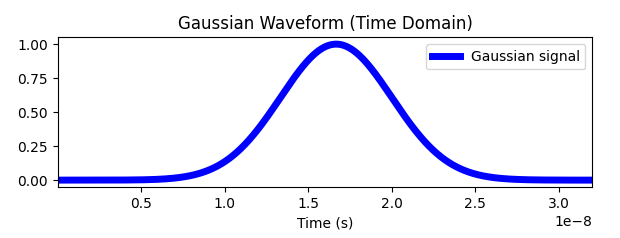
\includegraphics[width=15cm]{TFG/Metodologia/DFTgauss - arriba2.png}				
\caption{Gaussiana de prueba seleccionada en el dominio del tiempo.}
\end{figure}
\begin{figure}[H]
\centering
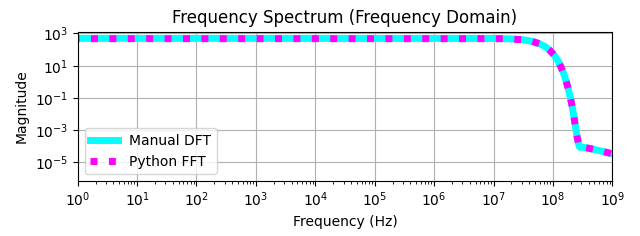
\includegraphics[width=15cm]{TFG/Metodologia/DFTgauss2_abajo.png}				
\caption{Comparativa entre la \textit{DFT} implementada y la \textit{FFT} de Python para la gaussiana seleccionada.}
\end{figure}
En este caso se ha elegido una gaussiana siguiendo la expresión (\ref{gauss1}) con $x_0=\frac{5}{c}\;m$ y $s_0=\frac{1}{c}\;m$ en un intervalo de frecuencias entre $10^0 \; Hz$ y $10^9\; Hz$.

Como se puede observar, ambas transformadas solapan completamente, lo que quiere decir que la implementación es correcta.

Una vez implementada la \textit{DFT}, y pudiendo ver cuánto decae la gaussiana en el dominio de la frecuencia en el que se trabaja, esta se elegirá de tal forma que decaiga en magnitud en menos de $10^{-2}$ con respecto al máximo de la magnitud original. La elección específica de valores se realizará en el apartado de resultados debido a que irá ligada al intervalo de frecuencias en el que se trabaje para el caso específico.

\subsection{Cálculo de \textit{R} y \textit{T}}
El punto clave del estudio será la obtención de los coeficientes de reflexión ($R$) y de transmisión ($T$) de las ondas electromagnéticas de forma correcta. Serán estos coeficientes los que dicten si el método simulado está implementado correctamente o no. En este apartado se explicará el cálculo de estos, así como su implementación.

Las distintas simulaciones que se realizarán consisten en una onda plana con forma de gaussiana evolucionando electromagnéticamente en el espacio de simulación. Este espacio estará diseñado de forma que la onda señal inicial se mueva a través del vacío hasta llegar a una \textit{lámina} o \textit{slab} la cual tendrá un grosor determinado y estará compuesta de un material específico con una permitividad y conductividad características.  Al toparse con dicha lámina, parte de la onda se reflejará al incidir sobre el \textit{slab} y otra parte se transmitirá. Posteriormente, la parte transmitida viajará en el interior del \textit{slab} volviendo a producirse una reflexión y transmisión al llegar a la superficie frontera del \textit{slab} con el vacío, repitiéndose este proceso hasta que la onda decaiga totalmente como consecuencia de la dispersión generada por viajar por un material con cierta conductividad, o bien la onda que se transmita al exterior del \textit{slab} alcance las fronteras computacionales del problema, halladas en los extremos del espacio, las cuales tienen definidas condiciones absorbentes de frontera de Silver-Müller (SM-ABC) \cite{SMA}. 

Para medir la amplitud reflejada y transmitida se escogen dos nodos. Considerando que nuestra onda plana inicial va a viajar en la dirección positiva $+x$, la elección del punto \textit{R} (Reflejado) será tal que la presencia de la gaussiana inicial no excite el campo eléctrico o magnético definido en el punto y se encuentre a la izquierda de dicha onda plana. Similarmente, el punto \textit{T} (Transmitido) se encontrará situado después de la lámina. El problema se dejará evolucionar hasta que se considere que la energía introducida por la onda plana en el sistema haya decrecido considerablemente, bien sea por la disipación introducida por la conductividad en el interior de la lámina o debido a que la onda ha sido absorbida en las fronteras computacionales, y se dará por concluida la medición de los valores de campo tanto en el punto \textit{R} como en el punto \textit{T}.

A continuación se exponen cuatro gráficas distintas en las que se muestra la evolución del campo eléctrico en ciertos pasos temporales en un medio con una lámina de características $d=20\;cm$, $\varepsilon=6$ y $\rho=8$ (se discutirá en el apartado \ref{ap412} el porqué de la adimensionalidad de la permitividad y resistividad):


\begin{figure}[H]
    \centering
    \begin{subfigure}[b]{0.45\textwidth}
        \centering
        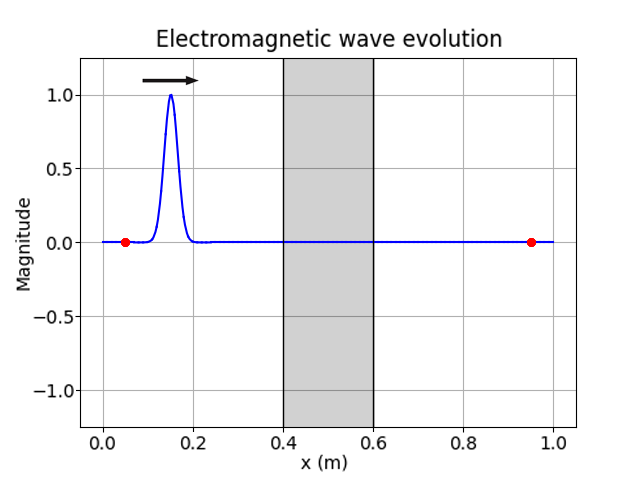
\includegraphics[width=\textwidth]{TFG/Metodologia/evolucion1d.png}
        \caption{La onda comienza a avanzar.}
        \label{f:gato}
    \end{subfigure}
    \hfill
    \begin{subfigure}[b]{0.45\textwidth}
        \centering
        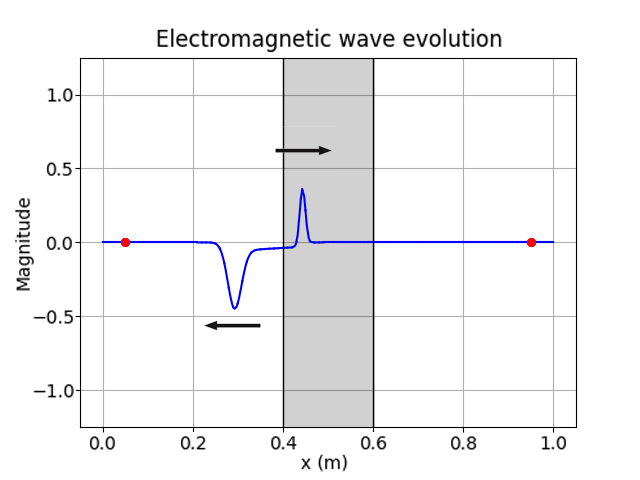
\includegraphics[width=\textwidth]{TFG/Metodologia/evolucion2d.png}
        \caption{Llega al \textit{slab} y se transmite y refleja.}
        \label{f:tigre}
    \end{subfigure}
    \begin{subfigure}[b]{0.45\textwidth}
        \centering
        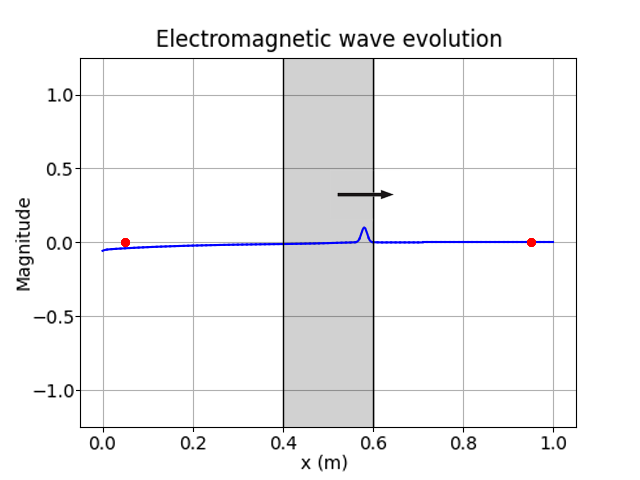
\includegraphics[width=\textwidth]{TFG/Metodologia/evolucion3d.png}
        \caption{La parte transmitida atraviesa el \textit{slab} mientras que la reflejada se absorbe.}
        \label{f:gato}
    \end{subfigure}
    \hfill
    \begin{subfigure}[b]{0.45\textwidth}
        \centering
        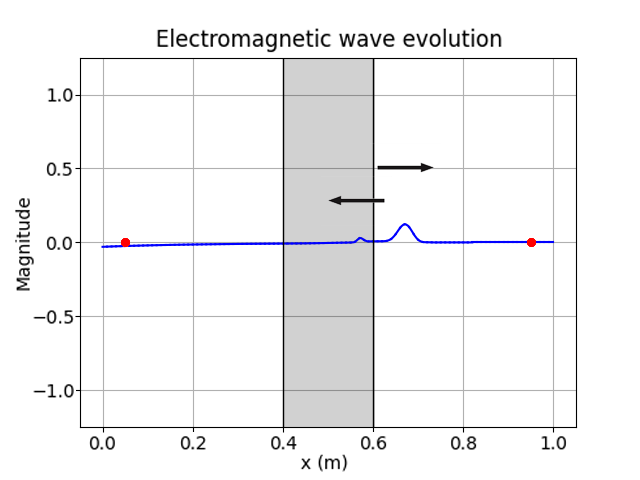
\includegraphics[width=\textwidth]{TFG/Metodologia/evolucion4d.png}
        \caption{La onda se refleja y transmite de nuevo.\\}
        \label{f:tigre}
    \end{subfigure}
    \caption{Simulación de la evolución de una onda electromagnética por un espacio con una lámina con $d=20\;cm$, $\varepsilon=6$ y $\rho=8$. El vídeo de esta simulación se puede ver en \cite{youtube}.}
    \label{fig5}
\end{figure}

Una vez se tienen guardados los campos que han pasado por los nodos correspondientes como transmitido y reflejado, calcular los coeficientes de transmisión y reflexión es sencillo. El primer paso para calcular los coeficientes se trata de pasar los campos al dominio de la frecuencia, que es con lo que trabajaremos. Para ello, tal y como se explicó en el apartado anterior, se realiza la \textit{DFT} tanto a la onda señal de entrada como a la reflejada y la transmitida. Una vez hecho, se aplican las siguientes expresiones:
\begin{equation}
    R=\frac{DFT(E_R)}{DFT(E_0)} \notag
\end{equation}
\begin{equation}
    T=\frac{DFT(E_T)}{DFT(E_0)} \notag
\end{equation}
donde $E_R$ es el campo acumulado en el nodo de la reflexión, $E_T$ el acumulado en el nodo de la transmisión y $E_0$ el campo de la señal inicial. Además, tanto el coeficiente de reflexión como el de transmisión en estas expresiones se realizan para cada frecuencia escogida dentro del intervalo que se elija.
%Explicación de la DFT
\newpage
\section{Resultados} \label{resultados}
%Muestro mis gráficas y las comparo con las de scikit y lo discuto.

Una vez se ha establecido el modelo y se ha implementado el código, se pueden realizar distintas simulaciones con el fin de verificar que la implementación es correcta. Para realizar esta validación se utilizará la librería de \textit{Scikit-rf} \cite{scikit}, que permite realizar simulaciones con las mismas características que las implementadas en esta tesis.

Para realizar las simulaciones se han de diseñar las condiciones que representarán. Estas condiciones deben incluir: el rango de frecuencias sobre el que se trabajará, la onda señal del campo eléctrico inicial y el espacio por el que se desplazará la onda. Estas deberán ser las ``condiciones iniciales'' a establecer y que se discutirán a continuación.
\subsection{Diseño de la simulación}
\subsubsection{Rango de frecuencias y onda señal}
La elección del rango de frecuencias que estudiar es el primer paso a considerar. Esto se debe a que el resto de componentes de la simulación y el estudio girarán tomando esta elección como base y construyendo sobre ella. Por ello, en todas las distintas simulaciones se ha escogido un rango que sea plausible para el estudio sin buscar casos específicos. El rango de frecuencias escogido es de los $10^8 \;Hz$ a los $10^9 \;Hz$ o, en otras palabras, entre $0.1\;GHz$ y $1 \;GHz$.

Una vez se ha elegido el rango de frecuencias, se puede elegir una onda que no decaiga en magnitud en dicho rango, tal y como se explicó en el apartado \ref{subsection34}. Se busca entonces que la magnitud de la onda caiga en menos de $10^{-2}$. Llevando a cabo dicho estudio, se llega a una onda de la forma (\ref{gauss1}) con los parámetros mostrados en la tabla (\ref{tab1}):
\begin{table}[h]
\centering
\begin{tabular}{|c|c|}
\hline
\textbf{$x_0$ (cm)} & \textbf{$s_0$ (cm)} \\ \hline
15                  & 1.5                 \\ \hline
\end{tabular}
\caption{Parámetros de la gaussiana utilizada en las simulaciones.}
\label{tab1}
\end{table}

La elección de $x_0$ se basa simplemente en que la gaussiana no se encuentre muy cerca del punto donde se recoge la onda reflejada, para que no interfiera en la toma de dichos datos. Este punto se encuentra a los cinco centímetros del inicio de la simulación, como se tratará en el siguiente apartado, y, colocando el máximo de la onda en el centímetro quince, no habrá posible mezcla de señales.

El parámetro de la desviación estándar, $s_0$, es la clave a la hora de configurar la onda. Esto se debe a que representa la anchura de la onda, lo cual, una vez llevado al dominio de la frecuencia, influencia las frecuencias que excitaremos en nuestro problema. Por tanto, esta variable se ha elegido cuidadosamente para que decaiga lo mínimo posible en el rango de frecuencias elegido. Se muestra a continuación la gaussiana elegida junto a su \textit{DFT} para apreciar el decaimiento de la onda en el dominio de las frecuencias:
\begin{figure}[H]
\centering
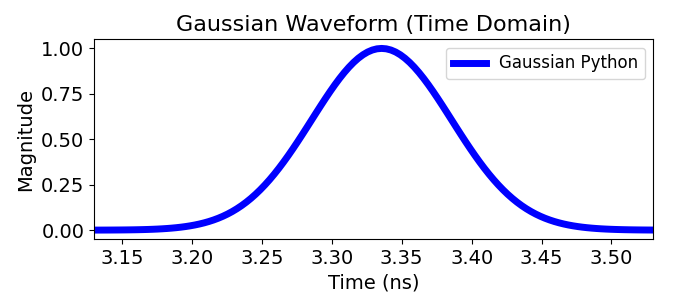
\includegraphics[width=15cm]{TFG/Resultados/onda6arriba.png}	
\caption{Representación de la onda elegida en el dominio del tiempo.}
\end{figure}

\begin{figure}[H]
\centering
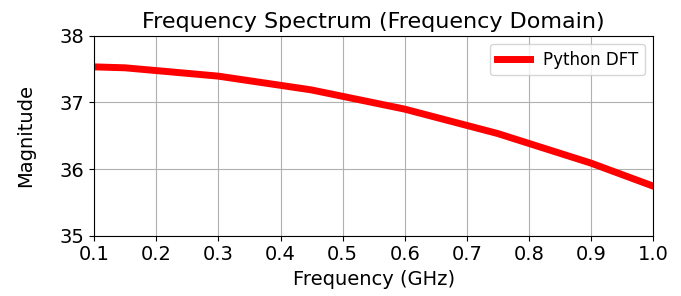
\includegraphics[width=15cm]{TFG/Resultados/onda6abajo.png}	
\caption{Decaimiento de la amplitud de la onda elegida en el dominio de la frecuencia.}
\end{figure}

Es claramente apreciable que la onda apenas decae, no llegando ni siquiera a acercarse a la caída de $10^{-2}$ que se había establecido como margen con respecto a la amplitud inicial. Podemos considerar, por tanto, una elección satisfactoria de los parámetros que definen nuestra gaussiana.

\subsubsection{Distribución espacial} \label{ap412}
Para observar el comportamiento de la onda frente a una reflexión y transmisión, se ha optado por hacer que la onda viaje por el vacío hasta encontrarse con el \textit{slab}, el cual tendrá unas características propias a elegir.

Lo primero es elegir el tamaño del espacio de simulación. Por estar tratando de un sistema unidimensional, el entorno de simulación debe tomar la forma de una línea recta. Se ha elegido que dicha recta tenga una longitud de \textbf{un metro} y esté conformada por \textbf{cien elementos}. Se toma un metro ya que, por cómo está normalizado el sistema de simulación, una unidad de longitud de la malla corresponde a un metro. A su vez, se elige dividir este espacio en 100 elementos, ya que, de esta forma, cada elemento tendrá una longitud de un centímetro. Esto se hace así porque facilita la distribución de los materiales en el espacio: si se quiere un \textit{slab} de un material de longitud cinco centímetros a una distancia de veinte centímetros del inicio del espacio, bastará con modificar las propiedades de cinco elementos a partir del elemento número veinte.

Consecuentemente, se debe definir qué es el vacío dentro de la simulación. Dentro del espacio de simulación estarán constituidos por vacíos aquellos elementos cuya conductividad sea 
\begin{center}
   $\sigma_0=0$ \;\; (S/m),
\end{center} 
y cuya permitividad sea 
\begin{center}
   $\varepsilon_0=8.85\cdot10^{-12}$\;\;(F/m).
\end{center} 
Estas son las propiedades del vacío en el mundo real, sin embargo, estas no serán las propiedades con las que se trabaje en la simulación. Si bien recordamos, se tomó como elección que el valor de la velocidad de la luz, $c$, fuese la unidad, de tal manera que $\epsilon_0$ y $\mu_0$, permitividad y permeabilidad del vacío, son iguales a la unidad también. Si continuamos desarrollando nuestros factores de conversión con respecto a estas definiciones, veremos que hemos de definir nuestras variables según las siguientes transformaciones:

\begin{equation}
    \varepsilon_{sim}=\frac{\varepsilon}{\varepsilon_0} \notag
\end{equation}
\begin{equation}
   \sigma_{sim}=\sigma\sqrt{\frac{\mu_0}{\varepsilon_0}}=\sigma Z_0=\frac{Z_0}{\rho} \notag
\end{equation}

donde $\mu_0= 4\pi \cdot 10^{-7}$ H/m, es decir, la permeabilidad del vacío, y $Z_0$ es la impedancia característica del vacío. Además, en la última ecuación se ha expresado la conductividad como $\sigma=\frac{1}{\rho}$ para facilitar la comparación con los resultados de la simulación de \textit{Scikit-rf}, ya que dicha librería opera con la resistividad, $\rho$, en vez de con la conductividad.

Aplicando estas transformaciones, el vacío en el espacio simulado tendrá las siguientes características:  $\varepsilon_{0,sim}$=1 y $\sigma_{0,sim}$=0, ambas en unidades normalizadas. De aquí en adelante se hablará en todo momento de unidades normalizadas para la simulación, que son las utilizadas a lo largo de los distintos casos.

Una vez se ha definido el vacío, queda establecer la distribución y propiedades de las láminas que se situarán en él. Se han diseñado dos experimentos con el fin de estudiar comportamientos distintos en el avance de la onda señal. El primero consiste en la introducción de una única lámina (N=1), la cual podrá adoptar distintas propiedades para un estudio más profundo del comportamiento. Para el segundo caso, en lugar de una única lámina, se colocarán tres láminas (N=3) equiespaciadas, estableciéndose vacío en el espacio de separación entre láminas.
\subsection{Estudio de la onda con una única lámina}
En este experimento se ha tomado un único \textit{slab} en el vacío. Los grosores de dicho \textit{slab}, $d$, se han variado entre uno y seis centímetros, quedando la situación inicial como en las siguientes representaciones:
\begin{figure}[H]
    \centering
        \begin{subfigure}[b]{0.475\textwidth}
        \centering
        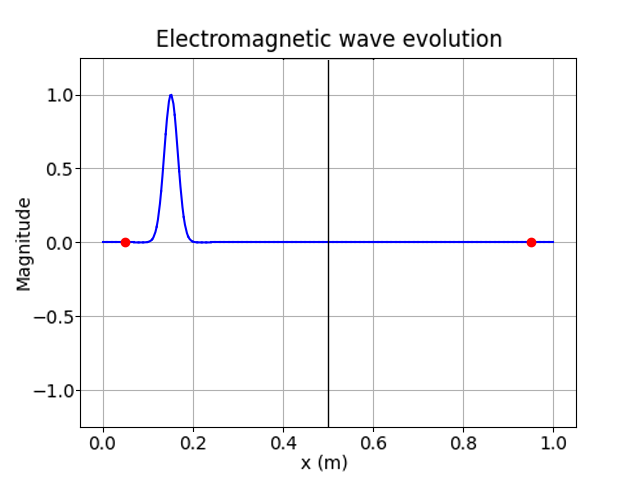
\includegraphics[width=\textwidth]{TFG/Resultados/initial state 1_13.png}
        \caption{d=1 cm}
        \label{f:gato}
    \end{subfigure}
    \hfill
    \begin{subfigure}[b]{0.475\textwidth}
        \centering
        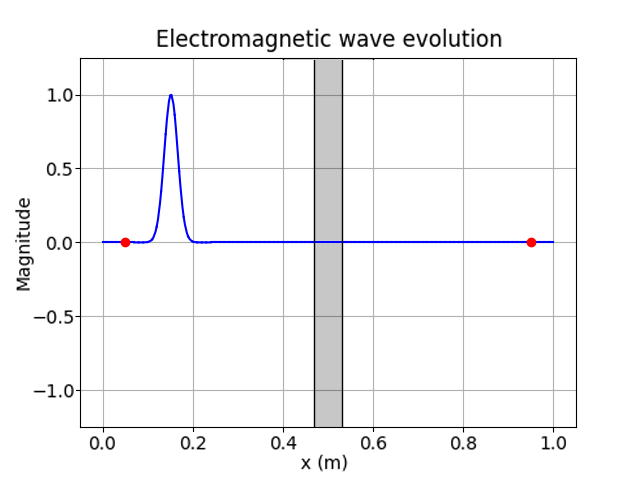
\includegraphics[width=\textwidth]{TFG/Resultados/initial state 1_63.png}
        \caption{d=6 cm}
        \label{f:tigre}
    \end{subfigure}
    \caption{Estado inicial de la simulación para N=1 con distintos grosores de lámina.}
    \label{fig5}
\end{figure}
Además, independientemente del grosor, también se han variado las distintas propiedades del material que conforma la lámina para cada caso. Es decir, se han buscado y estudiado casos en los cuales la conductividad y permitividad a lo largo del grosor del material hagan interesantes el estudio de los coeficientes de reflexión y transmisión.

Cabe destacar que para el estudio de los coeficientes de reflexión y transmisión se ha utilizado la magnitud de los mismos en decibelios. Para ello, se han realizado las siguientes transformaciones a los datos:
\begin{equation}
    R_{dB}=20\;log(R),\;\;\;\;\;\;\;\;\;\;\; T_{dB}=20\;log(T)\notag
\end{equation}
donde \textit{log} se interpreta como el logaritmo en base diez.

Finalmente, se muestran en la figura (\ref{fig9}) la representación de los resultados de la simulación realizada junto a los datos teóricos obtenidos mediante el uso de \textit{Scikit-rf} para las láminas escogidas.
\newpage
\begin{figure}[H]
    \centering
        \begin{subfigure}[b]{0.475\textwidth}
        \centering
        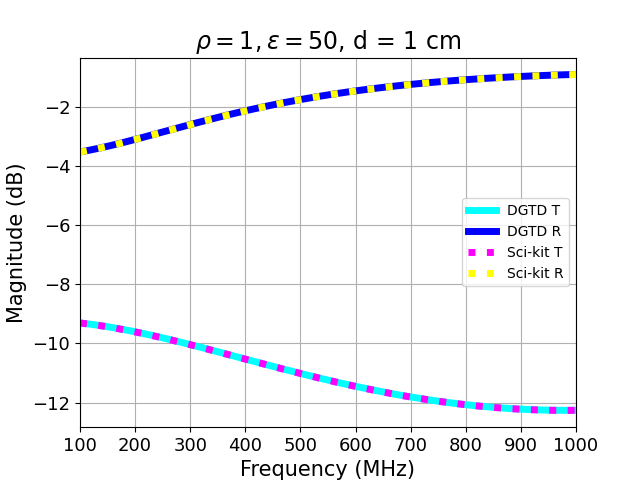
\includegraphics[width=\textwidth]{TFG/Resultados/single_50_1_12.png}
        \caption{$\rho$=1, $\varepsilon=50$, d=1 cm}
        \label{f:gato}
    \end{subfigure}
    \hfill
    \begin{subfigure}[b]{0.475\textwidth}
        \centering
        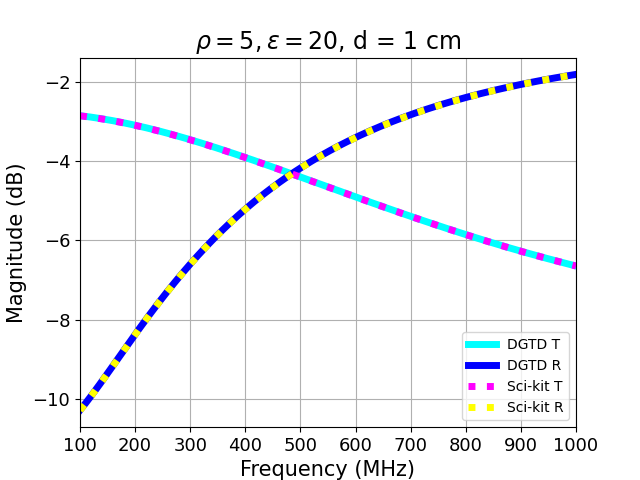
\includegraphics[width=\textwidth]{TFG/Resultados/single_20_5_12.png}
        \caption{$\rho$=5, $\varepsilon=20$, d=1 cm}
        \label{f:tigre}
    \end{subfigure}

        \begin{subfigure}[b]{0.475\textwidth}
        \centering
        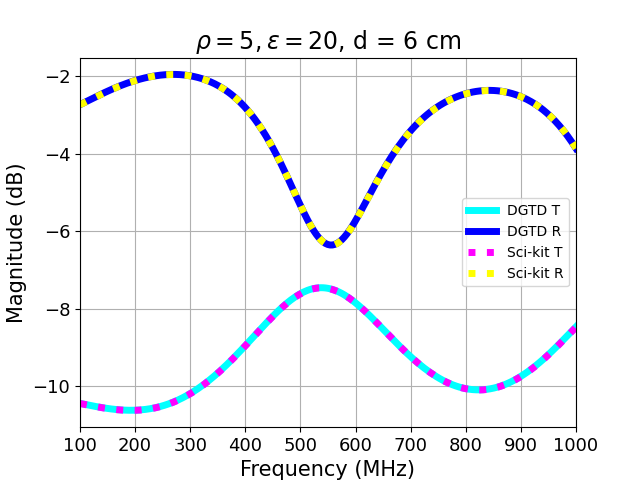
\includegraphics[width=\textwidth]{TFG/Resultados/single_20_5_62.png}
        \caption{$\rho$=5, $\varepsilon=20$, d=6 cm}
        \label{f:gato}
    \end{subfigure}
    \hfill
    \begin{subfigure}[b]{0.475\textwidth}
        \centering
        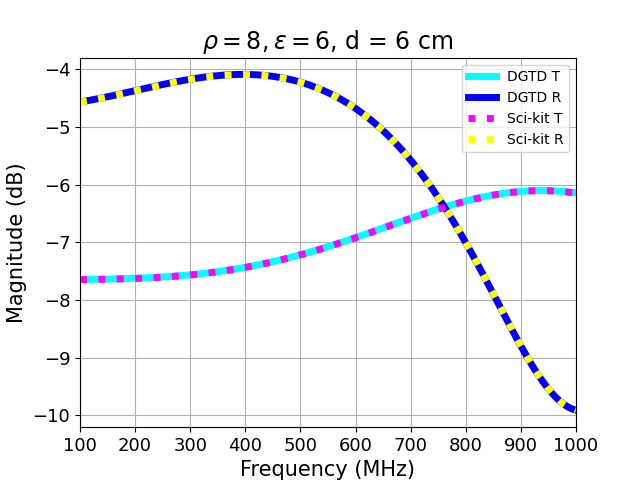
\includegraphics[width=\textwidth]{TFG/Resultados/single_6_8_62.png}
        \caption{$\rho$=8, $\varepsilon=6$, d=6 cm}
        \label{f:tigre}
    \end{subfigure}
    \caption{Comparativa de los resultados obtenidos para las simulaciones de N=1 con distintos parámetros $\rho$, $\varepsilon$ con los datos de \textit{Scikit-rf}.}
    \label{fig9}
\end{figure}
Como se puede ver en las gráficas y en los errores relativos calculados para estos casos, mostrados en las tablas (\ref{tab2}) y (\ref{tab3}), los resultados se adaptan perfectamente al marco teórico dado por \textit{Scikit-rf}, existiendo un error relativo mucho menor al $1\%$ en cada caso.
\begin{table}[H]
\centering
\begin{tabular}{|c|c|c|c|}
\hline
\textbf{$\epsilon_{r,R,(a)}$ ($\%$)} & \textbf{$\epsilon_{r,R,(b)}$ ($\%$)} & \textbf{$\epsilon_{r,R,(c)}$ ($\%$)} & \textbf{$\epsilon_{r,R,(d)}$ ($\%$)} \\ \hline
0.17                                 & 0.090                                & 0.13                                 & 0.063                                \\ \hline
\end{tabular}
\caption{Errores relativos medios de los coeficientes de reflexión obtenidos para N=1.}
\label{tab2}
\end{table}
\begin{table}[H]
\centering
\begin{tabular}{|c|c|c|c|}
\hline
\textbf{$\epsilon_{r,T,(a)}$ ($\%$)} & \textbf{$\epsilon_{r,T,(b)}$ ($\%$)} & \textbf{$\epsilon_{r,T,(c)}$ ($\%$)} & \textbf{$\epsilon_{r,T,(d)}$ ($\%$)} \\ \hline
0.026                                & 0.071                                & 0.038                                & 0.048                                \\ \hline
\end{tabular}
\caption{Errores relativos medios de los coeficientes de transmisión obtenidos para N=1.}
\label{tab3}
\end{table}
\newpage
\subsection{Estudio de la onda con múltiples láminas}
Una vez se ha comprobado que la simulación funciona correctamente con una lámina, independientemente del grosor, es interesante el estudio del comportamiento electromagnético de la onda al atravesar varias láminas para observar cómo evoluciona en un entorno más complejo. En la figura (\ref{fig10}) se muestra cuál será la distribución de los \textit{slabs} para este estudio.

\begin{figure}[H]
\centering
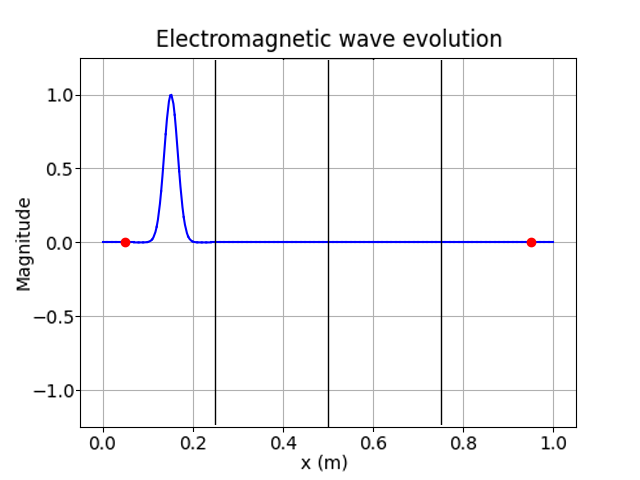
\includegraphics[width=11cm]{TFG/Resultados/initial state 32.png}	
\caption{Estado inicial de la simulación para N=3.}
\label{fig10}
\end{figure}

A continuación, al igual que para los distintos casos de una sola lámina, se muestran en la figura (\ref{fig11}) las comparativas de los coeficientes de reflexión y transmisión obtenidos por las simulaciones \textit{DG-FEM} frente a lo obtenido mediante \textit{Scikit-rf}.

De nuevo, aunque mirando las gráficas a simple vista es posible apreciar que los resultados obtenidos se superponen de forma casi completa a los teóricos, se ha calculado el error relativo medio, expuesto en las tablas (\ref{tab4}) y (\ref{tab5}). Este error relativo, una vez más, indica que la simulación y, por tanto, el código realizados son un éxito, teniendo esta vez un error relativo inferior al $0.1\%$ en todos los casos.
\newpage
\begin{figure}[H]
    \centering
        \begin{subfigure}[b]{0.475\textwidth}
        \centering
        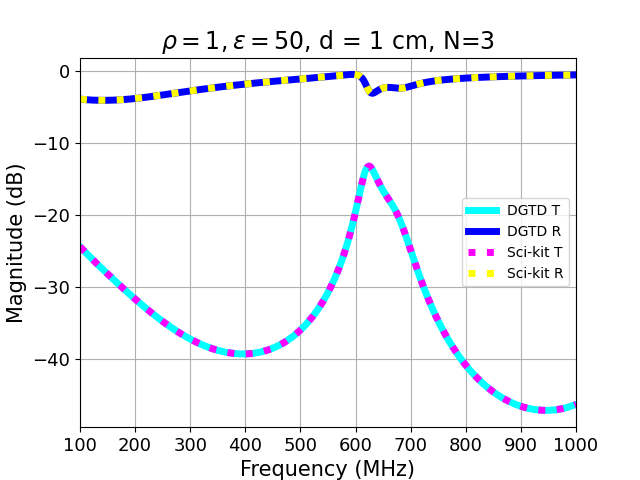
\includegraphics[width=\textwidth]{TFG/Resultados/50_12.png}
        \caption{$\rho$=1, $\varepsilon=50$, d=1 cm}
        \label{f:gato}
    \end{subfigure}
    \hfill
    \begin{subfigure}[b]{0.475\textwidth}
        \centering
        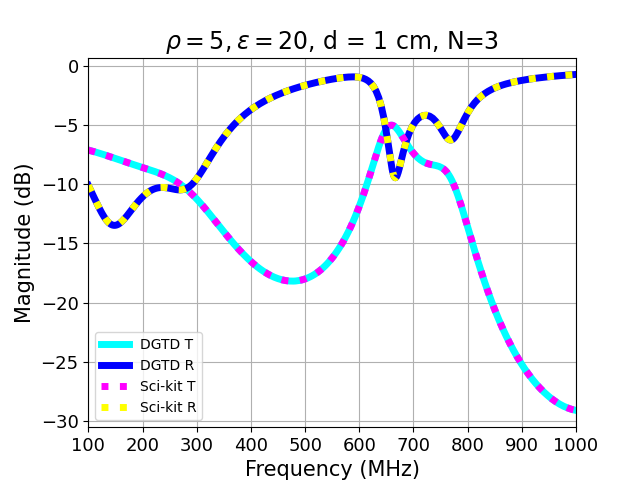
\includegraphics[width=\textwidth]{TFG/Resultados/20_52.png}
        \caption{$\rho$=5, $\varepsilon=20$, d=1 cm}
        \label{f:tigre}
    \end{subfigure}

        \begin{subfigure}[b]{0.475\textwidth}
        \centering
        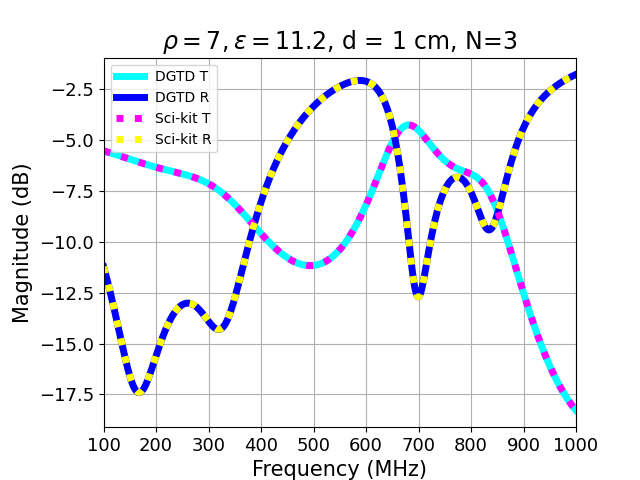
\includegraphics[width=\textwidth]{TFG/Resultados/112_72.png}
        \caption{$\rho$=7, $\varepsilon=11.2$, d=1 cm}
        \label{f:gato}
    \end{subfigure}
    \hfill
    \begin{subfigure}[b]{0.475\textwidth}
        \centering
        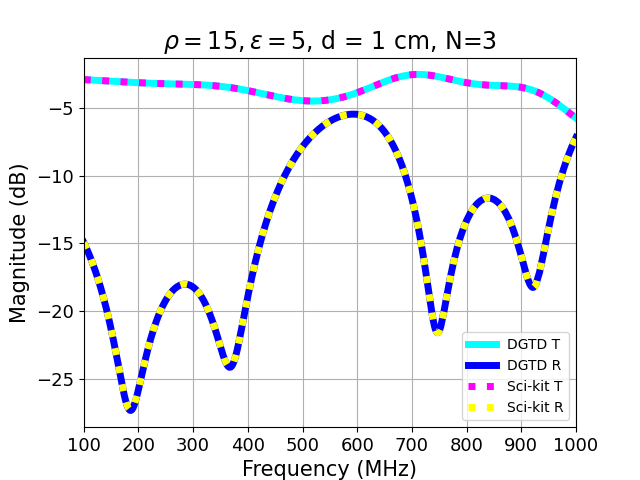
\includegraphics[width=\textwidth]{TFG/Resultados/5_152.png}
        \caption{$\rho$=15, $\varepsilon=5$, d=1 cm}
        \label{f:tigre}
    \end{subfigure}
    \caption{Comparativa de los resultados obtenidos para las simulaciones de N=3 con distintos parámetros $\rho$, $\varepsilon$ con los datos de \textit{Scikit-rf}.}
    \label{fig11}
\end{figure}
\begin{table}[H]
\centering
\begin{tabular}{|c|c|c|c|}
\hline
\textbf{$\epsilon_{r,R,(a)}$ ($\%$)} & \textbf{$\epsilon_{r,R,(b)}$ ($\%$)} & \textbf{$\epsilon_{r,R,(c)}$ ($\%$)} & \textbf{$\epsilon_{r,R,(d)}$ ($\%$)} \\ \hline
0.074                                 & 0.042                                & 0.060                                 & 0.034                                \\ \hline
\end{tabular}
\caption{Errores relativos medios de los coeficientes de reflexión obtenidos para N=3.}
\label{tab4}
\end{table}
\begin{table}[H]
\centering
\begin{tabular}{|c|c|c|c|}
\hline
\textbf{$\epsilon_{r,T,(a)}$ ($\%$)} & \textbf{$\epsilon_{r,T,(b)}$ ($\%$)} & \textbf{$\epsilon_{r,T,(c)}$ ($\%$)} & \textbf{$\epsilon_{r,T,(d)}$ ($\%$)} \\ \hline
0.019                                & 0.018                                & 0.022                                & 0.020                                \\ \hline
\end{tabular}
\caption{Errores relativos medios de los coeficientes de transmisión obtenidos para N=3.}
\label{tab5}
\end{table}

\newpage

\section{Conclusiones}

A lo largo de este \textit{Trabajo de Fin de Grado} se ha buscado entender e implementar un modelo capaz de simular el comportamiento de ondas electromagnéticas a través de distintos materiales. Para ello se consideraron diversos métodos numéricos que permitieran realizar dicha tarea, los cuales fueron: \textit{FDM}, \textit{FVM}, \textit{FEM} y \textit{DG-FEM}. El punto de partida para poder realizar esta elección fue el entendimiento de los estudios ya establecidos por Hesthaven \cite{Hesthaven} y Silvester \cite{Silvester}.

El estudio realizado a partir del trabajo de Hesthaven permitió profundizar en los conceptos necesarios para poder comprender y elegir entre los métodos numéricos considerados. La comprensión de estas explicaciones y las ventajas y desventajas que suponían los distintos métodos para los objetivos de esta tesis llevó a realizar la decisión fundamentada de escoger el método \textit{DG-FEM} como el más adecuado para los casos de estudio de este \textit{TFG}. 

Una vez se consiguió afianzar los conceptos fundamentales, se ha podido pasar a analizar el código desarrollado por el Grupo de Electromagnetismo de Granada de la Universidad de Granada (\textit{GEG-UGR}) \cite{repo}. A partir de esto, el foco de este \textit{TFG} ha sido la implementación en el código del \textit{GEG-UGR} de propiedades materiales tales como la permitividad ($\varepsilon$) y la densidad de carga ($\sigma$) en el ámbito unidimensional.

Todas las implementaciones realizadas se han validado como correctas en el apartado \ref{resultados} mediante el cálculo de los coeficientes de reflexión y transmisión para distintas configuraciones y condiciones iniciales. Cabe destacar que, ya que estas propiedades varían fundamentalmente según la frecuencia a la que se realicen los cálculos de reflexión y transmisión, para poder realizar un estudio que incluya  el comportamiento en un rango de frecuencias específico, dichos cálculos se han realizado en el dominio de la frecuencia mediante transformaciones discretas de Fourier de los resultados obtenidos en el dominio del tiempo. Para ello, se han diseñado varias simulaciones que giran alrededor del estudio de diversas configuraciones que contienen distintos números de \textit{láminas} o \textit{slabs} de diferentes materiales y grosores. Los coeficientes obtenidos de los datos proporcionados por las simulaciones se han comparado con los producidos por \textit{Scikit-rf} \cite{scikit}, software que ha proporcionado los datos que se han considerado como marco teórico a estudiar. Esta validación ha sido completamente satisfactoria, pudiendo observar en las tablas (\ref{tab2}), (\ref{tab3}), (\ref{tab4}) y (\ref{tab5}) errores relativos muy inferiores al 1$\%$ en todos los casos.

Se concluye, por tanto, que se han cumplido todos los objetivos propuestos, teniendo resultados que constatan la buena implementación de los modelos estudiados. La evolución natural de esta línea de investigación, de cara a futuro, sería la realización de estudios posteriores que busquen ampliar las bases ya establecidas en esta tesis a dos o más dimensiones.

% Referencias %%%%%%%%%%%%%%%%%%%%%%%%%%%%%%%%%%%%%%%%%%%%%%%%%%%%%%%%%%%%%%%%%
\newpage

\addcontentsline{toc}{section}{Referencias} % Elige según idioma
%\addcontentsline{toc}{section}{References} % Elige según idioma

\begin{thebibliography}{100}
\bibitem{abstract1}
%T. Hagstrom, D. Appelö and L. Zhang, "Discontinuous Galerkin Methods for Electromagnetic Waves in Dispersive Media," 2021 International Applied Computational Electromagnetics Society Symposium (ACES), Hamilton, ON, Canada, 2021, pp. 1-4.
  T.~Hagstrom, D.~Appelö  \& L.~Zhang, \\
  {\em Discontinuous Galerkin Methods for Electromagnetic Waves in Dispersive Media}, \\
  International Applied Computational Electromagnetics Society Symposium (ACES), Hamilton, ON, Canada, 2021.\\
  ISBN: 978-1-7335096-2-6

\bibitem{abstract2}
%Y. Wu, Z. Chen, W. Fan, J. Wang and J. Li, "A Wave-Equation-Based Spatial Finite-Difference Method for Electromagnetic Time-Domain Modeling," in IEEE Antennas and Wireless Propagation Letters, vol. 17, no. 5, pp. 794-798, May 2018, doi: 10.1109/LAWP.2018.2816678.
  Y.~Wu, Z.~Chen, W.~Fan, J.~Wang \& J.~Li, \\
  {\em A Wave-Equation-Based Spatial Finite-Difference Method for Electromagnetic Time-Domain Modeling}, \\
  in IEEE Antennas and Wireless Propagation Letters, vol. 17, no. 5, pp. 794-798, 2018.\\
  DOI: 10.1109/LAWP.2018.2816678

\bibitem{abstract3}
%Shankar, V., Mohammadian, A. H., & Hall, W. F. (1990). A Time-Domain, Finite-Volume Treatment for the Maxwell Equations. Electromagnetics, 10(1–2), 127–145. https://doi.org/10.1080/02726349008908232
  V.~Shankar, A.H.~Mohammadian \& W.F.~Hall, \\
  {\em A Time-Domain, Finite-Volume Treatment for the Maxwell Equations}, \\
  Electromagnetics, 10(1–2), 127–145, 1990.\\
  DOI: 10.1080/02726349008908232

  \bibitem{abstract4}
  C.~Clason, \\
  {\em Introduction to Finite Element Methods}, \\
  arXiv, 2021.\\
  DOI: 10.48550/arXiv.1709.08618

   \bibitem{scikit}
  %Scikit-rf Developers. (n.d.). scikit-rf: An open-source RF/Microwave engineering package for Python. https://scikit-rf.readthedocs.io/en/latest/
  Scikit-rf Developers, \\
  {\em scikit-rf: An open-source RF/Microwave engineering package for Python},\\  
$[$Computer software$]$.\\
 URL: \href{https://scikit-rf.readthedocs.io}{https://scikit-rf.readthedocs.io}

      \bibitem{computational}
%Dongarra, J., & Keyes, D. (2024). The co-evolution of computational physics and high-performance computing. Nature Reviews Physics. https://doi.org/10.1038/s42254-024-00750-z

  J.~Dongarra \& D.~Keyes, \\
  {\em The co-evolution of computational physics and high-performance computing},\\  
  Nature Reviews Physics, 2024. \\
  DOI: 10.1038/s42254-024-00750-z

  \bibitem{IEEComp}
 X.~Chunyan \& L.~Yu, \\
  {\em The Research of Electromagnetic Simulation Trusted Evaluation Technology Based on Super-Computing Platform},\\  
  International Applied Computational Electromagnetics Society Symposium (ACES-China), 2023. \\
  DOI: 10.23919/ACES-China60289.2023.10249826

    \bibitem{CompPhys}
 K.M.~Kiran Raj \textit{et al}, \\
  {\em Computational Physics Methods and Algorithms},\\ 
Journal of Physics: Conference Series, Volume 1712, International Conference On Computational Physics in Emerging Technologies (ICCPET), Mangalore, India, August 2020. \\
  DOI: 10.1088/1742-6596/1712/1/012028

    \bibitem{wikipedia}
  %Scikit-rf Developers. (n.d.). scikit-rf: An open-source RF/Microwave engineering package for Python. https://scikit-rf.readthedocs.io/en/latest/
  Wikipedia contributors, \\
  {\em Maxwell's equations},\\  
Wikipedia.\\
 URL: \href{https://en.wikipedia.org/wiki/Maxwell%27s_equations}{https://en.wikipedia.org/wiki/Maxwell's$\_$equations}

  
      \bibitem{intromaxwell}
 %Suárez, Á., Martí, A. C., Zuza, K., & Guisasola, J. (2022). Las relaciones causa-efecto en las ecuaciones de Maxwell y sus implicancias en la enseñanza del electromagnetismo en los cursos introductorios de Física. Revista Brasileira de Ensino de Física, 44(1), e20210289.

  A.~Suárez, A.C.~Martí, K.~Martí \& J.~Guisasola, \\
  {\em Las relaciones causa-efecto en las ecuaciones de Maxwell y sus implicancias en la enseñanza del electromagnetismo en los cursos introductorios de Física},\\  
  Revista Brasileira de Ensino de Física, 44(1), e20210289, 2022.\\
  DOI: 10.1590/1806-9126-RBEF-2022-0230

  \bibitem{numericos}
   F.M.~González Longatt, \\
  {\em Métodos numéricos para la solución de ecuaciones diferenciales: Un ejemplo comparativo},\\  
 Universidad Experimental Politécnica de la Fuerza Armada, 2006.\\
 URL: \href{https://fglongatt.org/OLD/Archivos/Archivos/SP_II/MetodoNumEDO.pdf}{https://fglongatt.org/OLD/Archivos/Archivos/SP$\_$II/MetodoNumEDO.pdf}
  %González-Longatt, F. M. (2006). Métodos numéricos para la solución de ecuaciones diferenciales: Un ejemplo comparativo. Universidad Experimental Politécnica de la Fuerza Armada. Recuperado de https://fglongatt.org/OLD/Archivos/Archivos/SP_II/MetodoNumEDO.pdf

    \bibitem{conservation}
  %Chirigati, F. From data to conservation laws. Nat Comput Sci 3, 733 (2023).
  F.~Chirigati, \\
  {\em From data to conservation laws},\\  
  Nature Computational Science, 3, 733, 2023.\\
  DOI: /10.1038/s43588-023-00524-0

 \bibitem{explicitorimplicit}
 %Živković, M., Milovanović, V., & Djordjević, N. (2009). Comparative analysis of implicit and explicit numerical methods in dynamic problems solving. En Proceedings of the 2nd International Congress of Serbian Society of Mechanics (IConSSM 2009) (pp. M2-28:1–12). Serbian Society of Mechanics.
   V.~Milovanović, M.~Živković\& N.~Djordjević, \\
  {\em Comparative analysis of implicit and explicit numerical methods in dynamic problems solving},\\ 
En Proceedings of the 2nd International Congress of Serbian Society of Mechanics (IConSSM 2009) (pp. M2-28:1–12). Serbian Society of Mechanics, 2009.\\
URL: \href{https://scidar.kg.ac.rs/handle/123456789/17706}{https://scidar.kg.ac.rs/handle/123456789/17706}

  \bibitem{repo}
%Silvester, P. P., & Ferrari, R. L. (1996). Finite elements for electrical engineers (3.ª ed.). Cambridge University Press.
  L.M.~Díaz Angulo, A.~Muñoz Manterola \& F.M.~Amador, \\
  {\em PyDG1D},\\  
    GitHub, 2024.\\
  $[$Computer software$]$.\\
  URL: \href{https://github.com/lmdiazangulo/PyDG1D}{https://github.com/lmdiazangulo/PyDG1D}

  
\bibitem{Hesthaven}
%Hesthaven, J. S., & Warburton, T. (2008). Nodal Discontinuous Galerkin Methods: Algorithms, Analysis, and Applications. Springer-Verlag New York.
  J.S.~Hesthaven \& T.~Warburton, \\
  {\em Nodal Discontinuous Galerkin Methods: Algorithms Analysis and Applications}, \\
  New York: Springer, 2008.\\
  DOI: 10.1007/978-0-387-72067-8
  


\bibitem{SMA}
L.M.~Díaz Angulo, \\
  {\em Time domain discontinuous Galerkin methods for Maxwell equations},\\  
 PhD Thesis, Universidad de Granada, 2014.\\
 URL: \href{http://hdl.handle.net/10481/35180}{http://hdl.handle.net/10481/35180}\\
 ISBN: 9788490832844
  %Díaz Angulo, L. M. (2014). Time domain discontinuous Galerkin methods for Maxwell equations [Tesis doctoral, Universidad de Granada]. Editorial Universidad de Granada. ISBN: 978-84-9083-284-4.

\bibitem{youtube}
P.~Valdés Gámiz, \\
 {\em Simulation for an electromagnetic wave travelling through a 20cm slab},\\  
 YouTube, 2025.\\ 
$[$Vídeo$]$.\\
 URL: \href{https://youtu.be/uwB9F_Kgdvc}{https://youtu.be/uwB9F$\_$Kgdvc}

 \bibitem{Silvester}
%Silvester, P. P., & Ferrari, R. L. (1996). Finite elements for electrical engineers (3.ª ed.). Cambridge University Press.
  P.~Silvester \& R.L.~Ferrari, \\
  {\em Finite elements for
electrical engineers},\\  
  Cambridge: Cambridge University Press, 1983.\\
  DOI: 10.1017/CBO9781139170611

 
 %   \bibitem{TM}
 %Wikipedia contributors. (n.d.). Transverse mode. Wikipedia. https://en.wikipedia.org/wiki/Transverse_mode
 % Wikipedia contributors, \\
 % {\em Transverse mode},\\  
%Wikipedia.\\
% URL: \href{https://en.wikipedia.org/wiki/Transverse_mode}{https://en.wikipedia.org/wiki/Transverse$\_$mode}.




\begin{comment}
\bibitem{charla}
  D.~Gross, \\
  {\em Quantum Field Theory: Past, Present and Future}, \\
  Talk at the Conference in Honour of the 90th Birthday of Freeman Dyson, \\
  Institute of Advanced Studies, Singapore, August 26-29, 2013.

\bibitem{libro}
  M.~E. Peskin and D.~V. Schroeder, \\
  {\em An Introduction to Quantum Field Theory}, \\
  Addison-Wesley, 1995.
  
\bibitem{tesis}
  M.~R.~Chala, \\
  {\em Collider Signatures of a Non-Standard Higgs Sector}, \\
  PhD Thesis, Universidad de Granada, 2014.

\bibitem{web}
 Particle Physics News and Resources, \\
 \href{http://www.interactions.org/}{http://www.interactions.org/}
\end{comment} 
\end{thebibliography}

\end{document}

